\documentclass[conference]{IEEEtran}
\usepackage{fontspec}
\usepackage{polyglossia}
\setdefaultlanguage{vietnamese}
\setotherlanguage{english}
\setmainfont{texgyretermes}[Extension=.otf, UprightFont=*-regular,
  BoldFont=*-bold, ItalicFont=*-italic, BoldItalicFont=*-bolditalic]
\usepackage{graphicx}
\usepackage{amsmath}
\usepackage{array}
\usepackage{xcolor}
% hyperref loads last so its patches of \ref, \label and \cite win.
\usepackage{hyperref}
\hypersetup{
  colorlinks=true,
  linkcolor=blue!60!black,
  citecolor=green!40!black,
  urlcolor=blue!60!black,
  pdftitle={Khai thác tập phổ biến bằng Eclat và hai ứng dụng thực tế},
  pdfauthor={Hung, Thien, Phat},
}
% Rows of the optimization-step table get labels so prose cites them with \ref.
\newcounter{optstep}
\newcommand{\optstep}[1]{\refstepcounter{optstep}\theoptstep\label{#1}}
\title{Khai thác tập phổ biến bằng Eclat và hai ứng dụng thực tế}
\author{\IEEEauthorblockN{Hung \and Thien \and Phat}
\IEEEauthorblockA{Nhóm DataMining — cập nhật họ tên và mã số sinh viên}}
\begin{document}
\maketitle
\begin{abstract}
Bản khung: bổ sung mục tiêu, phương pháp và kết quả sau khi hoàn tất thực nghiệm.
\end{abstract}
\section{Cài đặt}
Nhóm cài đặt lại Eclat từ bài báo gốc của Zaki~\cite{zaki2000} bằng Julia, chỉ dùng thư
viện chuẩn và không dùng thư viện khai thác tập phổ biến (frequent itemset mining, FIM)
nào. Gói có hai biến thể cho cùng một kết quả: bản cơ bản (baseline) bám sát bài báo, và
biến thể tối ưu (optimized). Chương này trình bày thuật toán và lý do nó cho kết quả đúng,
cách kiểm thử, các kỹ thuật tối ưu và mức cải thiện đo được so với bản cơ bản.

\subsection{Biểu diễn dọc và tidset}
Cơ sở dữ liệu (CSDL) gồm $N$ giao dịch (transaction). Mỗi giao dịch được gán một mã
giao dịch (transaction identifier, tid) là chỉ số $1, 2, \dots, N$ theo thứ tự đọc.
Apriori lưu CSDL theo chiều ngang (horizontal layout): mỗi giao dịch kèm danh sách item.
Eclat dùng biểu diễn dọc (vertical layout): mỗi item $x$ kèm tidset $t(x)$, tức tập mã
các giao dịch chứa $x$. Với itemset $X$, ta có
\begin{equation}
  t(X) = \{\, i \in \{1,\dots,N\} : X \subseteq T_i \,\}, \qquad
  \sigma(X) = |t(X)|,
  \label{eq:support}
\end{equation}
trong đó $T_i$ là giao dịch thứ $i$ và $\sigma(X)$ là độ hỗ trợ (support) của $X$, tức
số giao dịch chứa $X$. Itemset $X$ là phổ biến (frequent) khi
$\sigma(X) \ge \mathit{minsup}$, với $\mathit{minsup}$ là ngưỡng hỗ trợ tối thiểu tính
bằng số giao dịch. Giao dịch rỗng vẫn có tid và vẫn được tính vào $N$, nhưng không xuất
hiện trong tidset nào.

Bản cơ bản lưu mỗi tidset dưới dạng \texttt{Vector\{Int\}} tăng dần, gọi là tid-list.
Hàm \texttt{to\_class} đọc CSDL một lần và thêm tid theo thứ tự tăng dần, nên mọi
tid-list đều đã sắp xếp mà không cần sắp lại.

Ưu điểm chính của biểu diễn dọc là phép giao. Một giao dịch chứa $P \cup \{a, b\}$ khi
và chỉ khi nó chứa cả $P \cup \{a\}$ lẫn $P \cup \{b\}$, nên
\begin{equation}
  t(P \cup \{a, b\}) = t(P \cup \{a\}) \cap t(P \cup \{b\}),
  \label{eq:intersect}
\end{equation}
trong đó $P$ là một itemset và $a, b$ là hai item không thuộc $P$. Độ hỗ trợ của itemset
mới vì vậy được tính từ hai tidset sẵn có, không cần quét lại CSDL.

\subsection{Lớp tương đương theo tiền tố và tìm kiếm Bottom-Up}
Zaki chia không gian tìm kiếm thành các lớp tương đương theo tiền tố (prefix-based
equivalence class)~\cite{zaki2000}. Lớp có tiền tố (prefix) $P$ gồm các phần tử
$(b, t(P \cup \{b\}))$, với mỗi $b$ lớn hơn mọi item của $P$. Hai itemset trong cùng
một lớp chỉ khác nhau ở item cuối, nên phép giao~\eqref{eq:intersect} chỉ hợp lệ giữa
các phần tử cùng lớp.

Hàm \texttt{bottom\_up!} cài đặt thủ tục Bottom-Up của bài báo. Với mỗi phần tử $a$ của
lớp tiền tố $P$, hàm ghi $P \cup \{a\}$ cùng độ hỗ trợ, giao $t(P \cup \{a\})$ với tidset
của mọi phần tử $b$ đứng sau $a$, giữ lại các kết quả phổ biến làm lớp con có tiền tố
$P \cup \{a\}$, rồi duyệt lớp con đó trước khi xét phần tử kế tiếp. Lớp gốc có tiền tố
rỗng và gồm các item phổ biến. Bài báo cho phép duyệt dàn các lớp theo chiều sâu
(depth-first search, DFS) hoặc chiều rộng và báo cáo kết quả theo chiều rộng; nhóm chọn
chiều sâu để bộ nhớ chỉ giữ một lớp cho mỗi mức trên đường đi hiện tại. Bài báo cũng đếm
trước các 2-itemset phổ biến bằng một mảng tam giác trên CSDL ngang; bản cơ bản bắt đầu
phép giao từ các item đơn để một thủ tục xử lý mọi mức, còn biến thể tối ưu dùng lại
bước đếm này ở Mục~\ref{sec:optimized}. Bảng~\ref{tab:mapping} đối chiếu các thành phần
của bài báo với mã nguồn.

\begin{table}[t]
\centering
\small
\caption{Đối chiếu bài báo~\cite{zaki2000} với mã nguồn trong \texttt{src/algorithm/}}
\label{tab:mapping}
\begin{tabular}{>{\raggedright\arraybackslash}p{0.37\columnwidth}>{\raggedright\arraybackslash}p{0.53\columnwidth}}
\hline
Bài báo & Bản cơ bản; biến thể tối ưu \\
\hline
Tid-list của item (Mục 4.1) & \texttt{to\_class}; \texttt{bitset\_tidsets} \\
Lớp theo tiền tố (Mục 4.2) & vector các cặp (item, tid-list); vector các
\texttt{ClassMember\{T\}} \\
Bottom-Up (Mục 4.3.1 và 5.2, Hình 12) & \texttt{bottom\_up!}; \texttt{eclat\_search!} \\
Giao hai tid-list & \texttt{intersect\_tidlists}; \texttt{intersect\_bitsets!} và
\texttt{intersect\_lists!} \\
Đếm 2-itemset bằng mảng tam giác (Mục 5.1) & không dùng; \texttt{count\_pairs} \\
\hline
\end{tabular}
\end{table}

Bảng~\ref{tab:trace} truy vết thuật toán trên CSDL \texttt{baskets.txt} gồm bốn giao
dịch $T_1 = \{1,2,3\}$, $T_2 = \{1,2\}$, $T_3 = \{1,3\}$, $T_4 = \{2,3\}$ với
$\mathit{minsup} = 2$. Các tidset ban đầu là $t(1) = \{1,2,3\}$, $t(2) = \{1,2,4\}$ và
$t(3) = \{1,3,4\}$. Thuật toán ghi đúng sáu itemset phổ biến, và tập $\{1,2,3\}$ bị tỉa
vì chỉ xuất hiện trong $T_1$.

\begin{table}[t]
\centering
\caption{Truy vết Bottom-Up trên \texttt{baskets.txt} với $\mathit{minsup} = 2$}
\label{tab:trace}
\begin{tabular}{llll}
\hline
Tiền tố & Phép giao & Tidset & Kết quả \\
\hline
$\emptyset$ & -- & $t(1) = \{1,2,3\}$ & ghi $\{1\}$, $\sigma = 3$ \\
$\{1\}$ & $t(1) \cap t(2)$ & $\{1,2\}$ & giữ $2$ \\
$\{1\}$ & $t(1) \cap t(3)$ & $\{1,3\}$ & giữ $3$ \\
$\{1\}$ & -- & $t(12) = \{1,2\}$ & ghi $\{1,2\}$, $\sigma = 2$ \\
$\{1,2\}$ & $t(12) \cap t(13)$ & $\{1\}$ & tỉa, $1 < 2$ \\
$\{1\}$ & -- & $t(13) = \{1,3\}$ & ghi $\{1,3\}$, $\sigma = 2$ \\
$\emptyset$ & -- & $t(2) = \{1,2,4\}$ & ghi $\{2\}$, $\sigma = 3$ \\
$\{2\}$ & $t(2) \cap t(3)$ & $\{1,4\}$ & giữ $3$ \\
$\{2\}$ & -- & $t(23) = \{1,4\}$ & ghi $\{2,3\}$, $\sigma = 2$ \\
$\emptyset$ & -- & $t(3) = \{1,3,4\}$ & ghi $\{3\}$, $\sigma = 3$ \\
\hline
\end{tabular}
\end{table}

\subsection{Tính đúng đắn}
\label{sec:correctness}
Mọi lớp mà \texttt{bottom\_up!} nhận đều thỏa bốn bất biến (invariant): (i) mỗi tid-list
tăng dần và không lặp; (ii) các phần tử xếp tăng dần theo item và lớn hơn mọi item của
tiền tố; (iii) mỗi phần tử là phổ biến; (iv) tid-list của phần tử $b$ đúng bằng
$t(P \cup \{b\})$. Lớp gốc thỏa cả bốn khi được tạo. Lớp con lấy các phần tử đứng sau
$a$ nên giữ (i) và (ii); phép kiểm tra kích thước trước khi thêm cho (iii); đẳng
thức~\eqref{eq:intersect} cho (iv).

Từ đó suy ra ba tính chất. Thứ nhất, độ hỗ trợ được ghi là chính xác theo (iv)
và~\eqref{eq:support}. Thứ hai, không itemset nào bị ghi hai lần: theo (ii) mọi khóa
$(x_1, \dots, x_k)$ tăng ngặt, và nó chỉ được ghi khi lớp tiền tố
$(x_1, \dots, x_{k-1})$ duyệt tới $x_k$; mỗi lớp chỉ được tạo một lần. Thứ ba, kết quả
đầy đủ nhờ tính đơn điệu giảm (anti-monotone) của độ hỗ trợ: nếu $X \subseteq Y$ thì
$\sigma(X) \ge \sigma(Y)$, nên việc tỉa một itemset không phổ biến không làm mất tập cha
phổ biến nào. Quy nạp theo độ dài cho thấy lớp tiền tố $(x_1, \dots, x_{j-1})$ chứa
mọi item $y > x_{j-1}$ sao cho $(x_1, \dots, x_{j-1}, y)$ phổ biến, nên mọi itemset phổ
biến đều được ghi. Tài liệu \texttt{docs/eclat.md} trong repository trình bày chứng minh
đầy đủ.

\subsection{Độ phức tạp}
Gọi $L$ là tổng số item trên mọi giao dịch, $m$ là số item phân biệt và $C$ là số phép
giao. Dựng biểu diễn dọc tốn $O(L)$ thời gian kỳ vọng cho từ điển, $O(m \log m)$ để sắp
xếp và $O(L)$ bộ nhớ. Một phép giao tốn $O(|t(P \cup \{a\})| + |t(P \cup \{b\})|)$, tối
đa $O(N)$. Một lớp có $k$ phần tử thực hiện $k(k-1)/2$ phép giao, nên tổng thời gian là
\begin{equation}
  O(L + m \log m + C \cdot N),
  \label{eq:cost}
\end{equation}
với $C$ là tổng số phép giao trên mọi lớp được duyệt. Vì tìm kiếm theo chiều sâu, bộ nhớ
chỉ giữ các lớp trên đường đi hiện tại, mỗi mức một lớp gồm tối đa $m$ phần tử, mỗi
phần tử tối đa $N$ tid. Số kết quả có thể tăng theo hàm mũ: một $k$-itemset phổ biến có
$2^k - 1$ tập con khác rỗng, và mọi tập con đó đều phổ biến.

\subsection{Giao diện, định dạng SPMF và dòng lệnh}
Hai ứng dụng và phần thực nghiệm chỉ gọi bốn hàm công khai: \texttt{read\_transactions}
đọc file SPMF (mỗi dòng một giao dịch, các item cách nhau bởi dấu cách),
\texttt{support\_threshold} đổi $\mathit{minsup}$ thành số giao dịch, \texttt{mine} trả
về từ điển \texttt{SupportMap} từ itemset sang độ hỗ trợ, và \texttt{write\_itemsets}
ghi mỗi itemset một dòng theo dạng \texttt{1 2 \#SUP: 2}. Một $\mathit{minsup}$ thực
trong $(0, 1]$ là tỉ lệ và được làm tròn lên thành $\lceil \mathit{minsup} \cdot N \rceil$
giao dịch; một $\mathit{minsup}$ nguyên là số giao dịch tuyệt đối. Tham số
\texttt{variant} chọn \texttt{:baseline} hoặc \texttt{:optimized}, nên hai biến thể được
chọn riêng và so sánh trên cùng đầu vào.

Chương trình dòng lệnh \texttt{demo.jl} nhận đường dẫn đầu vào, \texttt{--output},
đúng một trong hai ngưỡng \texttt{--minsup} (tỉ lệ) hoặc \texttt{--min-count} (số giao
dịch) và \texttt{--variant}, ví dụ
\texttt{julia --project=. demo.jl --minsup 0.5 --output out.txt data/toy/baskets.txt}.
Đầu vào sai làm chương trình dừng với mã thoát 1 và thông báo nêu số dòng lỗi. Hàm ghi
kiểm tra toàn bộ kết quả trước khi mở tệp, nên một lần chạy lỗi không làm thay đổi tệp
đầu ra đã có. Các itemset được ghi theo thứ tự từ điển (lexicographic order) của mã item,
nên tệp đầu ra của hai biến thể giống nhau từng byte.

\subsection{Kiểm thử tự động}
\label{sec:tests}
Lệnh \texttt{julia --project=. test/runtests.jl} chạy 1\,091 phép kiểm tra, và tất cả
đều đạt trên Julia 1.13.2. Mỗi kiểm thử khai thác so sánh toàn bộ \texttt{SupportMap} lẫn
số itemset được ghi, vì một itemset bị ghi hai lần sẽ bị từ điển che mất. Cả hai biến thể
chạy cùng các nhóm kiểm thử sau.

\begin{itemize}
\item Kết quả tính tay: tám CSDL nhỏ, gồm CSDL rỗng, CSDL không có tập phổ biến, giao
dịch lặp và ngưỡng nằm ngay trên và dưới độ hỗ trợ của một itemset, và một CSDL ảnh có
giao dịch rỗng.
\item Đối chiếu với Eclat của SPMF~\cite{spmf2016}: tám lần chạy trên bảy CSDL nhỏ và
một lần chạy trên T25I10D10K (9\,976 giao dịch, 929 item), nơi SPMF cho 14\,782 itemset
dài từ 1 đến 13 item ở $\mathit{minsup} = 0{,}008$. Cả hai biến thể khớp 100\% trên cả
chín lần chạy, không có itemset thiếu, thừa hoặc sai độ hỗ trợ.
\item Đối chiếu với bộ đếm vét cạn (brute force) liệt kê mọi tập con: 10 CSDL ngẫu
nhiên sinh với hạt giống 42 cho mỗi biến thể. Biến thể tối ưu chạy thêm tám CSDL có 0, 1,
63, 64, 65, 127, 128 và 129 giao dịch, tức quanh biên của một từ 64 bit trong bitset; một
nửa trong số đó chứa các nhóm item luôn đi cùng nhau để sinh phần mở rộng hoàn hảo. Mỗi
CSDL chạy với 18 tổ hợp cấu hình bật và tắt từng kỹ thuật ở Mục~\ref{sec:optimized}.
\item Tính ổn định kiểu (type stability): \texttt{Test.@inferred} trên \texttt{mine},
\texttt{mine\_packed} và các hàm tìm kiếm của hai biến thể.
\item Đọc, ghi và dòng lệnh: hàm đọc theo byte được đối chiếu với bộ phân tích theo dòng
trên các đầu vào biên (số tràn \texttt{Int}, ký tự lạ, dòng trống, xuống dòng kiểu Windows)
và mọi CSDL nhỏ, hàm ghi được so từng byte với một bộ định dạng tham chiếu, và các lỗi tham
số cùng mã thoát của tiến trình được kiểm tra.
\end{itemize}

Bộ đếm vét cạn chỉ là công cụ kiểm thử. Ngoài bộ kiểm thử, mỗi đợt đo ở
Mục~\ref{sec:measure} so sánh mọi tệp đầu ra với một lần chạy Eclat của SPMF độc lập sau
khi đo xong. Đợt đo cuối gồm 820 tệp đầu ra trên năm CSDL chuẩn (615 của biến thể tối ưu
và 205 của PrePost+), và cả 820 tệp khớp 100\%.

\subsection{Biến thể tối ưu}
\label{sec:optimized}
Biến thể tối ưu giữ nguyên thủ tục Bottom-Up và thay đổi ba thứ: cách lưu tidset, những
phép giao được bỏ qua, và cách ghi kết quả. Mỗi thay đổi đều giữ đầu ra chính xác; các
chứng minh nằm trong \texttt{docs/eclat-optimized.md}. Phần khởi động, đọc và ghi tệp nằm
trong mã dùng chung, nên cả hai biến thể cùng hưởng các thay đổi ở đó.

\subsubsection{Tidset dạng bitset và thứ tự duyệt}
Ở ngưỡng thấp nhất của mỗi CSDL, lời gọi khai thác của bản cơ bản cấp phát 3{,}3 đến
5{,}7 GiB, chủ yếu cho tid-list mới của mỗi phép giao. Biến thể tối ưu lưu mỗi tidset
thành bitset (chuỗi bit, bit thứ $i$ ứng với giao dịch $i$) gồm $W = \lceil N/64 \rceil$
từ 64 bit. Phép giao là phép AND từng từ, và độ hỗ trợ là số bit 1 đếm bằng
\texttt{count\_ones} trong cùng vòng lặp. Kết quả được ghi vào một bitset lấy từ kho dùng
lại (pool); bitset của phép giao không phổ biến quay về kho, nên phép giao thất bại không
cấp phát bộ nhớ. Một phép giao đọc $2W$ từ bất kể độ hỗ trợ: $W = 50$ ở Chess và
$5\,316$ ở Accidents.

Các item được duyệt theo độ hỗ trợ tăng dần. Item hiếm đứng đầu được giao với nhiều item
nhất, nhưng hầu hết các phép giao đó thất bại, còn item phổ biến đứng cuối chỉ còn ít
phần tử theo sau, nên các lớp con nhỏ hơn. Chứng minh ở Mục~\ref{sec:correctness} chỉ
dùng một thứ tự toàn phần trên các item, nên nó vẫn đúng với thứ tự này.

\subsubsection{Tỉa phần mở rộng hoàn hảo và cấp phát kết quả một lần}
Một item $b$ là phần mở rộng hoàn hảo (perfect extension)~\cite{borgelt2012} của itemset
$X$ khi $t(X \cup \{b\}) = t(X)$, tức mọi giao dịch chứa $X$ đều chứa $b$. Vì
$t(X \cup \{b\}) \subseteq t(X)$, điều kiện này tương đương với hai độ hỗ trợ bằng nhau,
nên chỉ cần so sánh một số đếm. Khi đó mọi itemset $X \cup Y$ trong cây con của $X$ có
cùng độ hỗ trợ với $X \cup Y \cup S$, với $S$ là tập con bất kỳ của tập phần mở rộng
hoàn hảo $E$. Biến thể tối ưu vì vậy bỏ $b$ khỏi lớp con và không giao tidset của $b$
thêm lần nào. Mỗi nút (node) của cây tìm kiếm đại diện cho $2^{|E|}$ itemset có chung độ
hỗ trợ. Ở Mushroom 0{,}05, cây tìm kiếm chỉ có 33\,819 nút cho 3\,755\,511 itemset.

Phép tìm kiếm chỉ ghi lại các nút theo thứ tự duyệt trước (preorder), mỗi nút gồm độ
sâu, item nó thêm vào, các phần mở rộng hoàn hảo nó tìm thấy và độ hỗ trợ. Hàm
\texttt{expand\_nodes} tính kích thước cuối cùng của kết quả từ các nút, có kiểm tra tràn
số, cấp phát ba mảng kết quả đúng một lần, rồi ghi các tập con $S$ theo thứ tự mã Gray
(Gray code) để hai itemset liên tiếp chỉ khác nhau một item. Nếu để mảng kết quả lớn dần
theo từng itemset, mỗi lần gấp đôi dung lượng phải sao chép toàn bộ mảng: ở Mushroom
0{,}05, lời gọi khai thác trong một tiến trình đã khởi động (warm) cấp phát 1\,068 MiB để
tạo một kết quả 306 MiB và mất 0{,}40 s; khi cấp phát một lần, nó cấp phát 310 MiB và mất
0{,}17 s.

\subsubsection{Dữ liệu thưa: đếm cặp, danh sách tid và cận theo khối}
Trên dữ liệu thưa, phép giao bitset vẫn đọc đủ $W$ từ dù tidset ngắn ($W = 1\,378$ ở
Retail và $1\,563$ ở T10I4D100K), và hầu hết phép giao thất bại. Ở Retail 0{,}001,
99{,}9\% trong 2\,239\,786 phép giao ở lớp gốc không đạt ngưỡng. Ở T10I4D100K 0{,}00025,
phần lớn phép giao nằm ở độ sâu 2 (2\,256\,822 phép, 99{,}1\% thất bại) trên các tidset
chỉ khoảng 100 tid. Ba kỹ thuật sau xử lý hai dạng này.

\emph{Đếm cặp ở lớp gốc.} Hàm \texttt{count\_pairs} đếm độ hỗ trợ của mọi cặp item phổ
biến bằng một mảng tam giác gồm $m_f(m_f-1)/2$ ô qua một lượt duyệt CSDL ngang, như Mục
5.1 của bài báo~\cite{zaki2000}, với $m_f$ là số item phổ biến. Lớp gốc chỉ giao những cặp
đạt ngưỡng. Tại gốc tiền tố rỗng, nên số đếm của cặp $(a, b)$ đúng bằng $|t(\{a, b\})|$
và không phép giao phổ biến nào bị bỏ. Việc đếm chỉ chạy khi chi phí ước lượng của nó nhỏ
hơn một phần mười chi phí các phép giao ở gốc, tức khi
$10 \sum_i |T_i|(|T_i| - 1)/2 < W m_f(m_f-1)/2$. Retail và T10I4D100K thỏa điều kiện này;
Chess, Mushroom và Accidents, với giao dịch dài và ít item phổ biến, vẫn giao như trước.

\emph{Danh sách tid theo lớp.} Một lớp con gồm $k$ phần tử chuyển từ bitset sang danh
sách tid tăng dần khi
\begin{equation}
  kW + c\,(k - 1) \sum_{i=1}^{k} \sigma_i < W\,\frac{k(k-1)}{2},
  \label{eq:lists}
\end{equation}
trong đó vế phải là số từ mà các phép giao bitset của lớp phải đọc, $kW$ là chi phí
chuyển đổi, $\sigma_i$ là độ hỗ trợ của phần tử thứ $i$, và $c = 8$ là chi phí một bước
trộn tính theo số từ, chọn từ phép quét $c$ từ 2 đến 16 trên máy đo.
Quy tắc~\eqref{eq:lists} dựa trên độ dài tidset và $N$, không dựa trên tên CSDL. Phép trộn hai danh sách không có nhánh rẽ phụ
thuộc dữ liệu và dừng sớm khi số tid chung đã tìm cộng phần còn lại của danh sách ngắn hơn
không thể đạt $\mathit{minsup}$.

\emph{Cận theo khối.} Ở T10I4D100K 0{,}00025, 98{,}7\% trong 2\,076\,972 phép trộn vẫn
thất bại, trên hai danh sách có tổng cộng trung bình 126 tid. Trước khi duyệt một lớp danh
sách tid, chương
trình chia khoảng tid thành tối đa $K = 256$ khối có độ rộng là lũy thừa của 2 và đếm số
tid của mỗi phần tử trong từng khối. Với hai phần tử $X$ và $Y$ của lớp,
\begin{equation}
  \sigma(X \cup Y) \le \sum_{j=1}^{K} \min(c_{X,j}, c_{Y,j}),
  \label{eq:bound}
\end{equation}
trong đó $c_{X,j}$ và $c_{Y,j}$ là số tid của $X$ và $Y$ trong khối $j$, vì một tid chung
nằm trong đúng một khối và được đếm một lần cho mỗi phần tử. Phép trộn nào có cận nhỏ hơn
$\mathit{minsup}$ bị bỏ qua mà không đọc tid nào. Cận~\eqref{eq:bound} không bao giờ loại
một phép giao phổ biến, nên đầu ra không đổi. Giá trị $K = 256$ được chọn từ phép quét 64
đến 512 khối.

\subsubsection{Khởi động, đọc và ghi}
Các thay đổi trong mục này nằm trong mã dùng chung của hai biến thể. Ở ngưỡng cao, thời
gian chạy không nằm trong thuật toán. Một tiến trình \texttt{demo.jl}
của bản cơ bản trên Chess 0{,}9 mất 2{,}36 s, trong khi khởi động Julia chỉ mất 0{,}17 s;
phần còn lại là biên dịch JIT (just-in-time, biên dịch khi chạy). Nhóm chạy các hàm công
khai và phần xử lý dòng lệnh trên một CSDL nhỏ trong lúc Julia dựng package image, để mã
máy của chúng được lưu kèm gói. Phần xử lý dòng lệnh nằm trong gói (\texttt{src/cli.jl})
thay vì trong tệp script, vì mã của script không được lưu trong package image và phải
biên dịch lại 108{,}6 ms ở mỗi lần chạy. Một phép kiểm thử chạy \texttt{demo.jl} trong
tiến trình mới với \texttt{--trace-compile} và yêu cầu không phương thức nào phải biên
dịch.

Ở ngưỡng thấp trên dữ liệu dày, phần lớn thời gian nằm ở việc ghi kết quả. Bộ lấy mẫu
\texttt{Profile} trên Mushroom 0{,}05 cho thấy phép sắp xếp đầu ra bằng so sánh chiếm
64\% thời gian, định dạng và ghi tệp 25\%, còn khai thác chỉ 11\%. Biến thể tối ưu duyệt
item theo độ hỗ trợ nên phải sắp lại kết quả theo thứ tự từ điển; nhóm thay phép sắp xếp
này bằng radix sort (sắp xếp theo cơ số) trên khóa 128 bit chứa các item đầu của itemset
và chỉ số của nó. Hàm ghi lấy chữ số của mỗi số nhỏ hơn $2^{20}$ từ một bảng tra và ghi
bằng một lệnh 8 byte. Hàm đọc phân tích mỗi dòng vào một vector dùng lại và sao chép một
lần với độ dài cuối cùng, nên lời gọi đọc Accidents (34 MB) trong một tiến trình đã khởi
động giảm từ 0{,}57 s còn 0{,}29 s và cấp phát 151 MiB thay vì 354 MiB.

\subsubsection{Đặc trưng của Julia}
Kiểu \texttt{ClassMember\{T\}} có tham số \texttt{T} là \texttt{UInt64} cho bitset hoặc
\texttt{Int} cho danh sách tid. Hàm tìm kiếm \texttt{eclat\_search!} được viết một lần,
và multiple dispatch (chọn phương thức theo kiểu của mọi đối số) chọn phép giao, quy tắc
chuyển đổi và bộ lọc phép giao theo \texttt{T}. Julia biên dịch một bản chuyên biệt cho
mỗi dạng tidset, nên vòng lặp trong không có phép kiểm tra kiểu khi chạy. Nhóm dùng
\texttt{Vector\{UInt64\}} thay cho \texttt{BitVector} vì vòng lặp giao ghi kết quả vào
vùng nhớ dùng lại và đếm bit trong cùng một lượt.

Kiểu khóa \texttt{Tuple\{Vararg\{Int\}\}} của \texttt{SupportMap} không cố định độ dài,
nên việc tạo hàng triệu khóa tốn hơn chính bước khai thác: trong một phép thử ban đầu trên
Mushroom 0{,}05, chèn 3{,}76 triệu itemset vào từ điển mất 12{,}4 s trong khi đếm độ hỗ trợ
của chúng mất 0{,}63 s. Cả hai biến thể vì vậy ghi kết
quả vào ba mảng \texttt{Vector\{Int\}} phẳng (item, vị trí bắt đầu của mỗi itemset, độ hỗ
trợ); hàm ghi tệp đọc thẳng ba mảng này, và \texttt{mine} chỉ dựng \texttt{SupportMap} ở
biên giao diện cho ứng dụng. Mọi hằng số điều chỉnh là \texttt{const}, mọi container trên
đường nóng có kiểu phần tử cụ thể. \texttt{@inbounds} chỉ có mặt ở phép trộn danh sách
tid và hàm ghi số, kèm chú thích chứng minh chỉ số hợp lệ. Trên vòng lặp giao bitset,
\texttt{@inbounds @simd} làm thời gian khai thác thay đổi từ $-8\%$ đến $+11\%$ trên năm
điểm đo, nằm trong nhiễu, nên nhóm không dùng.

\subsection{Đo lường mức cải thiện}
\label{sec:measure}
Mọi số đo trong mục này là trung vị thời gian của năm tiến trình \texttt{demo.jl} nguội
(cold), tức mỗi lần chạy là một tiến trình mới gồm khởi động Julia, đọc, khai thác và ghi
tệp. Các đợt đo chạy trên một máy Linux (Intel Core i7-11800H, 7{,}4 GiB RAM, xung nhịp
cố định 2{,}3 GHz) với Julia 1.13.2 một luồng. Lưới đo gồm 33 ngưỡng trên năm CSDL Chess,
Mushroom, Retail, T10I4D100K và Accidents, cùng một số ngưỡng stress thấp hơn lưới, chỉ
dùng để kiểm tra giới hạn. Ngoài Eclat của SPMF, nhóm so sánh với PrePost+~\cite{deng2015}
của \href{https://github.com/NgTHung/Itemset/blob/main/tools/spmf/release.toml}{bản SPMF đã ghim}
(Java Temurin 25.0.4.1, heap 4 GiB), vì đây là thuật toán nhanh hơn Eclat
của SPMF trên dữ liệu dày. Tỉ số $R = T_\text{tối ưu} / T_\text{PrePost+}$ chia trung vị
thời gian của biến thể tối ưu cho trung vị của PrePost+ ở cùng ngưỡng.

Mỗi kỹ thuật được đo trong một phiên riêng, trong đó phiên bản trước và sau thay đổi chạy
xen kẽ ở mỗi lần lặp, nên độ trôi của máy chia đều cho cả hai. Riêng bước tiền biên dịch
được đo bằng hai đợt liên tiếp. Bảng~\ref{tab:steps} cho tỉ số thời gian sau trên trước
của từng bước trên 33 ngưỡng, và tỉ số bộ nhớ đỉnh tương ứng. Bộ nhớ đỉnh là peak RSS
(resident set size, lượng bộ nhớ vật lý lớn nhất mà tiến trình chiếm) do hệ điều hành đo.

\begin{table*}[t]
\centering
\small
\caption{Tác động của từng bước tối ưu trên 33 ngưỡng: tỉ số thời gian và bộ nhớ đỉnh sau
trên trước (nhỏ hơn 1 là tốt hơn), và ngưỡng cải thiện nhiều nhất}
\label{tab:steps}
\begin{tabular}{rllll}
\hline
Bước & Kỹ thuật & Tỉ số thời gian & Ví dụ, thời gian trước $\to$ sau (s) & Tỉ số bộ nhớ \\
\hline
\optstep{step:precompile-package} & Tiền biên dịch các hàm của gói & 0{,}14 đến 0{,}83 & Chess 0{,}9: 2{,}36 $\to$ 0{,}33 & 0{,}82 đến 0{,}97 \\
\optstep{step:bitset} & Bitset và thứ tự độ hỗ trợ tăng dần & 0{,}10 đến 0{,}97 & Mushroom 0{,}1: 6{,}28 $\to$ 0{,}88 & 0{,}68 đến 0{,}99 \\
\optstep{step:perfect-extension} & Tỉa phần mở rộng hoàn hảo & 0{,}93 đến 1{,}04 & Mushroom 0{,}1: 0{,}89 $\to$ 0{,}83 & 0{,}95 đến 1{,}00 \\
\optstep{step:radix-sort} & Radix sort cho thứ tự ghi & 0{,}77 đến 1{,}02 & Mushroom 0{,}1: 0{,}83 $\to$ 0{,}64 & 1{,}00 đến 1{,}02 \\
\optstep{step:precompile-cli} & Tiền biên dịch dòng lệnh & 0{,}66 đến 0{,}94 & Chess 0{,}9: 0{,}33 $\to$ 0{,}22 & 0{,}91 đến 1{,}03 \\
\optstep{step:pair-count} & Đếm cặp ở lớp gốc & 0{,}24 đến 1{,}01 & Retail 0{,}001: 1{,}72 $\to$ 0{,}42 & 1{,}00 đến 1{,}03 \\
\optstep{step:tid-lists} & Danh sách tid theo lớp & 0{,}83 đến 1{,}02 & T10I4D100K 0{,}00025: 1{,}46 $\to$ 1{,}21 & 1{,}00 đến 1{,}01 \\
\optstep{step:byte-io} & Đọc và ghi theo byte, bảng chữ số & 0{,}76 đến 0{,}99 & Accidents 0{,}65: 1{,}10 $\to$ 0{,}85 & 0{,}74 đến 1{,}00 \\
\optstep{step:single-allocation} & Cấp phát kết quả một lần, cận theo khối & 0{,}82 đến 1{,}03 & T10I4D100K 0{,}00025: 1{,}18 $\to$ 0{,}97 & 0{,}83 đến 1{,}02 \\
\hline
\end{tabular}
\end{table*}

Bước~\ref{step:bitset} có tác động lớn nhất: thời gian còn 10\% đến 97\% của bản cơ bản (trung vị 37\%)
và bộ nhớ đỉnh giảm ở mọi ngưỡng. Bước~\ref{step:pair-count} chỉ tác động lên dữ liệu thưa, nơi nó giảm thời
gian của Retail 0{,}001 đi 76\%. Bước~\ref{step:perfect-extension} một mình chỉ rút ngắn tối đa 6{,}9\% thời gian
tiến trình, vì ở ngưỡng đó việc sắp xếp và ghi hàng trăm nghìn itemset chiếm phần lớn thời
gian; nhóm vẫn giữ bước này vì nó không làm tăng bộ nhớ và là nền của bước~\ref{step:single-allocation}. Không bước
nào làm một ngưỡng chậm đi quá 4{,}4\%.

Bảng~\ref{tab:final} cho tác động cộng dồn của các bước~\ref{step:bitset}
đến~\ref{step:single-allocation} ở ngưỡng cao nhất và thấp nhất của mỗi CSDL: nó so sánh bản
cơ bản sau bước~\ref{step:precompile-package} với biến thể tối ưu sau
bước~\ref{step:single-allocation}. Các bước~\ref{step:precompile-cli} và~\ref{step:byte-io}
nằm trong mã dùng chung, nên bản cơ bản của phiên bản nộp cũng hưởng hai bước này; phép so
sánh hai biến thể trên cùng một phiên bản mã là bước~\ref{step:bitset} của
Bảng~\ref{tab:steps}. Hai cột được đo ở hai phiên cách nhau ba ngày trên cùng máy và cùng
cấu hình. PrePost+ chạy trong cả hai phiên, và trung vị của nó giữa hai phiên lệch nhau từ
$-3{,}8\%$ đến $+5{,}8\%$ (trung vị $+0{,}3\%$), nên hai phiên so sánh được với nhau trong
sai số này.

\begin{table*}[t]
\centering
\small
\caption{Trung vị thời gian tiến trình nguội (s) và bộ nhớ đỉnh lớn nhất (MiB) trong năm
lần chạy. Bản cơ bản (sau bước~\ref{step:precompile-package}) đo ngày 06/11/2026, biến thể
tối ưu (sau bước~\ref{step:single-allocation}) và
PrePost+ ngày 09/11/2026, Eclat của SPMF ngày 31/10/2026, cùng một máy}
\label{tab:final}
\begin{tabular}{lrrrrrrrr}
\hline
 & & \multicolumn{5}{c}{Thời gian (s)} & \multicolumn{2}{c}{Bộ nhớ đỉnh (MiB)} \\
Dữ liệu / minsup & Itemset & Cơ bản & Tối ưu & Tăng tốc & Eclat SPMF & PrePost+ & Cơ bản & Tối ưu \\
\hline
Chess / 0{,}9 & 622 & 0{,}33 & 0{,}21 & 1{,}6 & 0{,}51 & 0{,}42 & 268 & $\le 254$ \\
Chess / 0{,}6 & 254\,944 & 3{,}24 & 0{,}30 & 10{,}8 & 15{,}98 & 0{,}59 & 308 & 262 \\
Mushroom / 0{,}5 & 153 & 0{,}33 & 0{,}22 & 1{,}5 & 0{,}51 & 0{,}44 & 256 & $\le 254$ \\
Mushroom / 0{,}1 & 574\,431 & 6{,}28 & 0{,}40 & 15{,}7 & 7{,}44 & 0{,}68 & 414 & 302 \\
Retail / 0{,}01 & 159 & 0{,}55 & 0{,}29 & 1{,}9 & 1{,}19 & 0{,}80 & 304 & $\le 254$ \\
Retail / 0{,}001 & 7\,589 & 12{,}80 & 0{,}38 & 33{,}5 & 1{,}53 & 3{,}52 & 331 & 281 \\
T10I4D100K / 0{,}01 & 385 & 2{,}93 & 0{,}32 & 9{,}1 & 0{,}78 & 1{,}42 & 304 & $\le 254$ \\
T10I4D100K / 0{,}00025 & 96\,959 & 10{,}92 & 0{,}97 & 11{,}3 & 8{,}02 & 4{,}34 & 363 & 279 \\
Accidents / 0{,}95 & 15 & 1{,}31 & 0{,}78 & 1{,}7 & 4{,}59 & 1{,}71 & 650 & 397 \\
Accidents / 0{,}65 & 1\,093 & 7{,}13 & 0{,}86 & 8{,}3 & 26{,}87 & 2{,}34 & 804 & 397 \\
\hline
\end{tabular}
\end{table*}

Trên cả 33 ngưỡng, các bước~\ref{step:bitset} đến~\ref{step:single-allocation} rút ngắn thời gian tiến trình từ 1{,}5 đến 33{,}5 lần
(trung vị 4{,}0 lần). Trung bình nhân của mức tăng tốc theo CSDL là 3{,}1 lần ở Accidents,
3{,}3 ở Mushroom, 3{,}4 ở Chess, 6{,}5 ở Retail và 13{,}5 ở T10I4D100K. Mức tăng nhỏ nhất
nằm ở các ngưỡng cao của Chess và Mushroom, nơi một lần chạy chỉ còn khoảng 0{,}22 s, trong
đó 0{,}19 s là khởi động Julia và nạp gói; ở đó phần lớn mức tăng đến từ bước~\ref{step:precompile-cli}. So với
SPMF, biến thể tối ưu nhanh hơn Eclat từ 2{,}3 đến 53 lần, theo số đo Eclat của phiên
31/10/2026, và nhanh hơn PrePost+ ở cả 33 ngưỡng, với $R$ từ 0{,}11 đến 0{,}59. Trung bình
nhân của $R$ theo CSDL là 0{,}20 ở Retail, 0{,}21 ở T10I4D100K, 0{,}41 ở Accidents, 0{,}49
ở Mushroom và 0{,}51 ở Chess. Độ trải tứ phân vị (interquartile range, IQR) của hai cột
Cơ bản và Tối ưu không vượt quá 3{,}3\% trung vị ở mọi ngưỡng.

Bộ nhớ đỉnh sau bước~\ref{step:single-allocation} thấp hơn bản cơ bản ở mọi ngưỡng. Mức giảm lớn nhất nằm ở
Accidents (804 còn 397 MiB ở 0{,}65), nhờ hàm đọc không cấp phát thừa và tidset trong lúc
tìm kiếm chỉ chiếm vài MiB. Trên máy đo, cả ba chương trình Julia, Eclat và PrePost+ của
SPMF đều cho giá trị nhỏ nhất trong khoảng 253{,}0 đến 253{,}6 MiB, nên phép đo có một mức
sàn chung và các ô ghi $\le 254$ trong Bảng~\ref{tab:final} chỉ là cận trên.

Ba kỹ thuật đã được thử, đo và không giữ lại. Diffset~\cite{zaki2003} lưu các tid mà
một phần tử thiếu so với tiền tố; trong phép quét tỉ số chuyển đổi, không giá trị nào
nhanh hơn bitset, Accidents 0{,}2 chậm đi tới 10\% và T10I4D100K 0{,}00025 chậm đi tới
71\%. Lý do là phép tỉa phần mở rộng hoàn hảo đã loại mọi phần tử có diffset rỗng, đúng
những chỗ diffset có lợi nhất: ngay cả khi chọn tối ưu cho từng lớp, số từ cần đọc chỉ
giảm tối đa 0{,}3\%. In itemset trực tiếp từ khóa sắp xếp chậm hơn 5\% đến 7\%. Chỉ thị
\texttt{@inbounds @simd} trên phép giao bitset không cho mức cải thiện vượt nhiễu.

Biến thể tối ưu còn ba giới hạn đo được. Thứ nhất, ở ngưỡng stress Mushroom 0{,}05 chương
trình phải ghi 3\,755\,511 dòng và vẫn chậm hơn PrePost+ (1{,}45 s so với 1{,}38 s). Thứ
hai, mỗi tiến trình mất khoảng 0{,}19 s để khởi động Julia và nạp gói, phần này chỉ có thể
bỏ đi nếu biên dịch trước toàn bộ chương trình thành tệp thực thi. Thứ ba, đếm cặp làm bộ
nhớ đỉnh tăng 20\% ở ngưỡng stress Retail 0{,}00025, vì mảng tam giác cho 5\,918 item phổ
biến chiếm 67 MiB.

\section{Experiments and evaluation}
\label{sec:evaluation}
\subsection{Data and shared protocol}
\label{sec:protocol}
We ran the experiments on five standard benchmark databases from the FIM community:
Chess, Mushroom, Retail, T10I4D100K, and Accidents, all originally from the FIMI
repository~\cite{fimi}. Table~\ref{tab:datasets} lists statistics we computed from the
data files themselves: $N$ is the number of transactions, $|I|$ the number of distinct
items, $\bar{w}$ the mean transaction length, and the density $d = \bar{w} / |I|$ the
average fraction of all items that appear in a transaction. Chess and Mushroom are dense
($d \ge 0.19$), while Retail and T10I4D100K are sparse ($d \le 0.012$). Accidents falls
between the two groups with $d = 0.072$, but we count it as dense because its long
transactions ($\bar{w} = 33.81$, close to Chess) make its output grow as fast as that of
the dense databases (Section~\ref{sec:output-size}).

\begin{table}[t]
\centering
\caption{Statistics of the five benchmarks, computed from SHA-256-checked files}
\label{tab:datasets}
\begin{tabular}{lrrrrr}
\hline
Data & $N$ & $|I|$ & $\bar{w}$ & $w_{\max}$ & $d$ \\
\hline
Chess & 3\,196 & 75 & 37.00 & 37 & 0.493 \\
Mushroom & 8\,124 & 119 & 23.00 & 23 & 0.193 \\
Retail & 88\,162 & 16\,470 & 10.31 & 76 & 0.0006 \\
T10I4D100K & 100\,000 & 870 & 10.10 & 29 & 0.0116 \\
Accidents & 340\,183 & 468 & 33.81 & 51 & 0.072 \\
\hline
\end{tabular}
\end{table}

We identify each file by its SHA-256 hash rather than by its name, because the same name
can refer to different versions. For example, the \texttt{mushrooms.txt} file on the SPMF
site has 8\,416 transactions, whereas the FIMI version used by most papers has 8\,124; we use the FIMI version. Retail contains the anonymized receipts of a
Belgian retail store~\cite{brijs1999}, and Accidents contains records of injury traffic
accidents in Flanders, Belgium~\cite{geurts2003}. The SPMF copies of Chess and Accidents
are byte-identical to the FIMI ones. The FIMI versions of Retail and T10I4D100K, however,
contain item 0, which SPMF does not accept, so for these two we use the SPMF versions, in
which every item code is shifted up by 1. Renaming items this way leaves the support of
every itemset unchanged. Before any file is used, the script
\texttt{experiments/prepare\_benchmarks.jl} downloads the data again and checks its hash
and statistics.

A relative minsup is converted to the transaction count
$\sigma_{\min} = \lceil \mathrm{minsup} \cdot N \rceil$. During the experiments we found
that SPMF computes this product in 64-bit floating point: with $\mathrm{minsup} = 0.07$
and $N = 100$, SPMF requires $\sigma_{\min} = 8$, while exact decimal arithmetic gives
$\sigma_{\min} = 7$. The experiment runner therefore rejects any threshold on which the two
computations disagree, so that a difference between the two implementations can only come
from the algorithm.

Every attempt runs in a fresh process with a timeout and is recorded as CSV rows with a
fixed set of fields: dataset and hash, minsup and $\sigma_{\min}$, Git revision, algorithm
variant, environment, seed, time, peak memory, itemset count, and status. A failed or
timed-out attempt is kept with its status and is never replaced by a zero. Time is
reported in two scopes. The \emph{process} scope measures the whole process, including
Julia start-up and JIT compilation or JVM start-up. The \emph{mine} scope measures only the
call to \texttt{mine} after a warm-up run on a small database, so it contains no
compilation time. For SPMF we also record the time that SPMF reports itself. Peak memory
is the peak RSS (Section~\ref{sec:measure}) that the operating system reports through
\texttt{getrusage}; we use it because it is the only quantity that can be compared between
a Julia process and a Java process.

Every measurement in this paper ran on the benchmark machine: Linux, an Intel Core
i7-11800H with its clock fixed at 2.3\,GHz, 7.4\,GiB RAM, single-threaded Julia 1.13.2,
and the pinned SPMF release~\cite{spmf2016} on Java Temurin 25.0.4.1 with a 4\,GiB heap.
We treat SPMF as a black box: we report how its programs behave but do not attribute the
differences to causes inside them.

\subsection{Correctness against SPMF}
\label{sec:exact}
Two implementations can report the same number of itemsets and still disagree on their
supports, so counting itemsets is not enough. We use SPMF's Eclat as an independent
reference and compare the full map from itemset to support count. The comparator skips
metadata lines and sorts the items inside each key, so the order in which itemsets are
printed does not matter. The match rate is the number of keys that appear exactly once on
each side with the same support, divided by the number of distinct keys in the union of
the two outputs; two empty maps count as a full match. Missing, extra, duplicate, and
wrong-support keys are reported separately.

On the eight comparisons of the test suite on seven small databases, the baseline reaches
100\% with no missing, extra, duplicate, or wrong-support itemset
(Table~\ref{tab:toy-spmf} in Appendix~\ref{app:toy}). On the five benchmarks, we checked every output of the runtime campaign of
Section~\ref{sec:minsup}, which ran both variants at revision \texttt{ca60f43} five times
on each of 33 database and threshold pairs, against one independent SPMF Eclat result per
pair. All 330 outputs of the two variants reach a 100\% match rate, with no missing,
extra, duplicate, or wrong-support itemset. Table~\ref{tab:bench-exact} gives the number
of matching thresholds for each variant together with the range of SPMF output sizes, and
Fig.~\ref{fig:exact-grid} shows which minsup values were checked.

\begin{figure}[t]
\centering
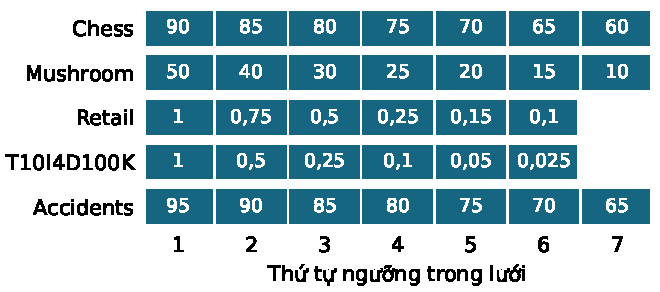
\includegraphics[width=\columnwidth]{figures/correctness-grid.pdf}
\caption{Minsup grid per database. Each cell gives minsup as a percentage and marks a
point where both variants match SPMF on every itemset and support.}
\label{fig:exact-grid}
\end{figure}

\begin{table}[t]
\centering
\caption{Thresholds whose full output matches SPMF, and the number of reference itemsets}
\label{tab:bench-exact}
\begin{tabular}{lrrr}
\hline
Data & Baseline & Optimized & Itemset range \\
\hline
Chess & 7/7 & 7/7 & 622--254\,944 \\
Mushroom & 7/7 & 7/7 & 153--574\,431 \\
Retail & 6/6 & 6/6 & 159--7\,589 \\
T10I4D100K & 6/6 & 6/6 & 385--96\,959 \\
Accidents & 7/7 & 7/7 & 15--1\,093 \\
\hline
\end{tabular}
\end{table}

\subsection{Runtime against minimum support}
\label{sec:minsup}
We timed four programs in a single session on the benchmark machine
(Section~\ref{sec:protocol}): the baseline, the optimized variant, SPMF 2.67 Eclat, and
SPMF PrePost+. Both Julia variants ran through the \texttt{demo.jl} command-line
interface at the same revision (\texttt{ca60f43}), so all times are in the
\emph{process} scope (Section~\ref{sec:protocol}). The grid covers 33 (benchmark, minsup) points
on the five benchmarks of Table~\ref{tab:datasets}, each repeated five times, and every
one of the 660 runs matched an independent SPMF Eclat run itemset for itemset.

Each point is the median of its five repeats. Relative to the median, the interquartile
range is at most 2.9\% for the baseline, 1.9\% for the optimized variant, 11.3\% for SPMF,
and 13.9\% for PrePost+. Because the four programs ran in the same session, we treat a
ratio as a real difference when it exceeds about 5\% between the two Julia variants and
about 16\% when one side is a Java program; Appendix~\ref{app:noise} derives these margins
and the drift between sessions.

\begin{figure*}[t]
\centering
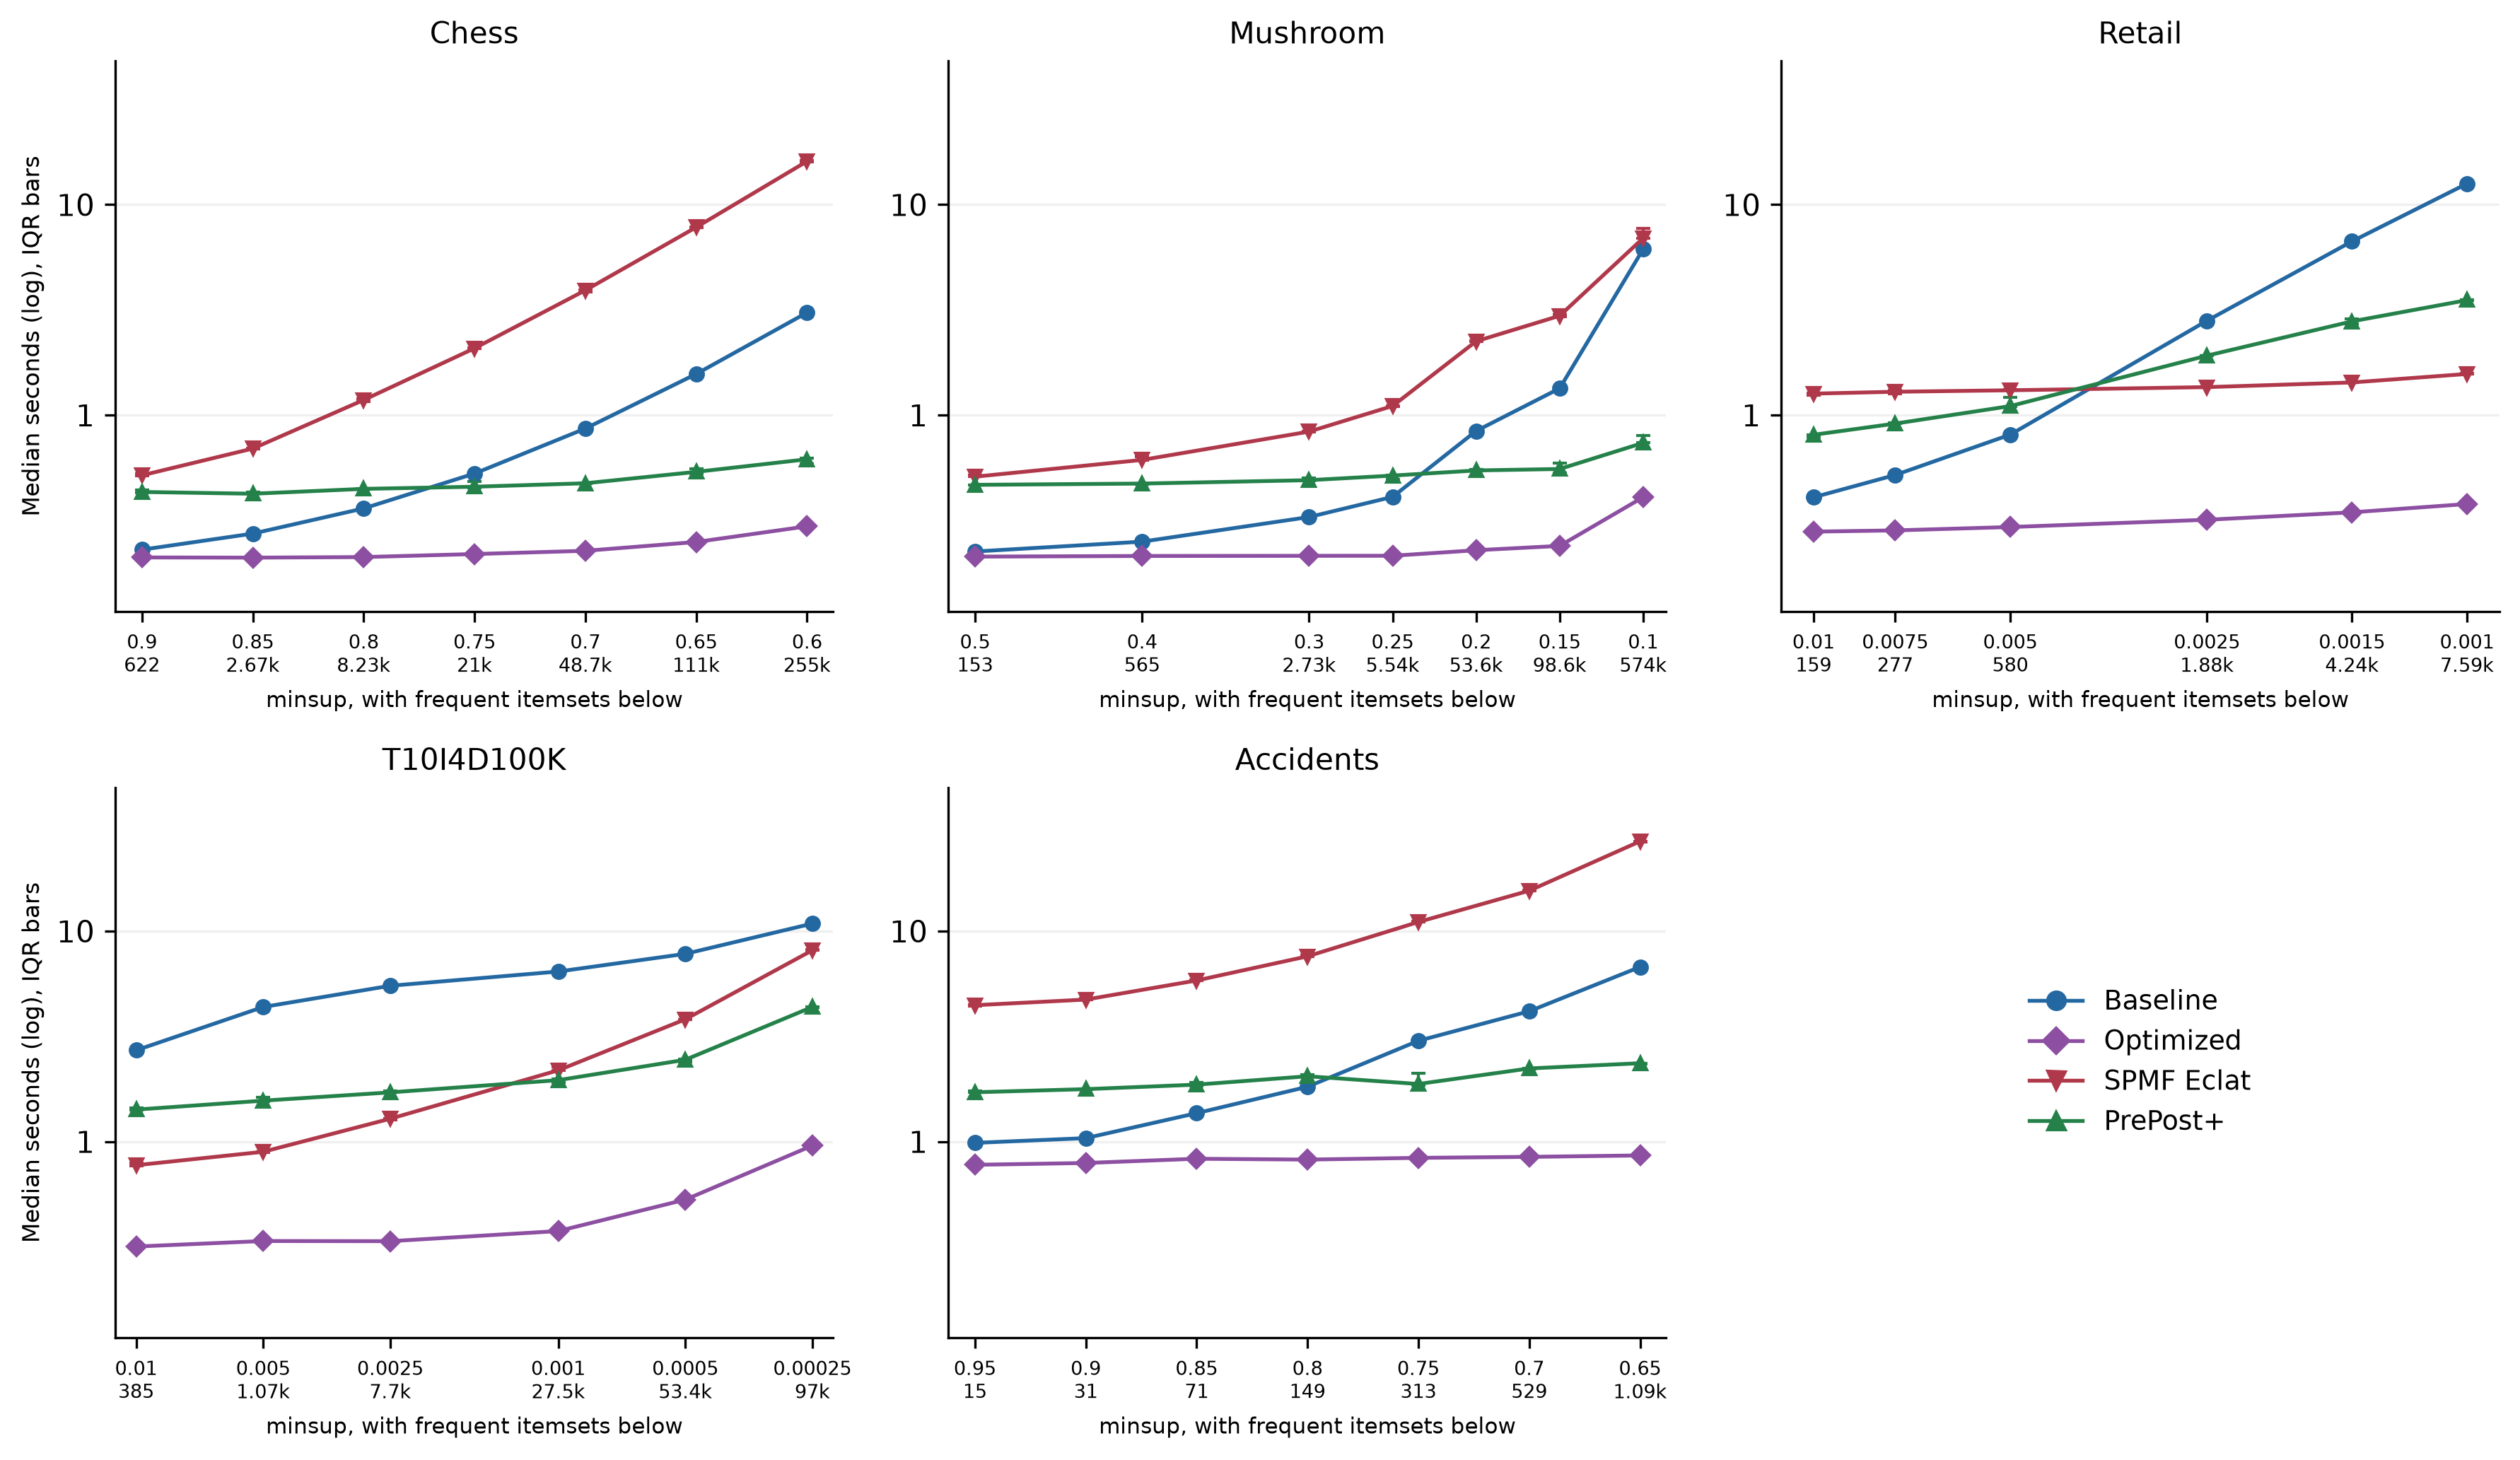
\includegraphics[width=\textwidth]{figures/runtime-curves.png}
\caption{\emph{Process} time against minsup for the four programs on the five
benchmarks. The vertical axis is logarithmic, points are medians of five repeats, and bars
are interquartile ranges. Below each horizontal-axis label is the number of frequent
itemsets.}
\label{fig:runtime}
\end{figure*}

The optimized variant is the fastest program at all 33 points, taking between 0.21 and
0.96\,s. At the lowest minsup of each benchmark (Table~\ref{tab:runtime-low}) it beats the
baseline by a factor of about 7.9 on Accidents, 10.4 on Chess, 11.3 on T10I4D100K, 15.1
on Mushroom, and 33.3 on Retail. Table~\ref{tab:runtime-ratio} in
Appendix~\ref{app:ratios} gives the geometric mean of this ratio over all points of each
benchmark, along with the same ratio for SPMF Eclat and PrePost+.

\begin{table}[t]
\centering
\footnotesize
\setlength{\tabcolsep}{3pt}
\caption{\emph{Process} time (seconds) at the lowest minsup of each benchmark, median of
five repeats. ``Sets'' is the number of frequent itemsets, and ``SPMF'' is SPMF's Eclat.}
\label{tab:runtime-low}
\begin{tabular}{lrrrrrr}
\hline
Data / minsup & Sets & Baseline & Optimized & SPMF & PrePost+ \\
\hline
Chess / 0.6 & 254\,944 & 3.07 & 0.30 & 16.07 & 0.62 \\
Mushroom / 0.1 & 574\,431 & 6.15 & 0.41 & 6.93 & 0.74 \\
Retail / 0.001 & 7\,589 & 12.59 & 0.38 & 1.57 & 3.52 \\
T10I4D100K / 0.00025 & 96\,959 & 10.86 & 0.96 & 8.11 & 4.36 \\
Accidents / 0.65 & 1\,093 & 6.76 & 0.86 & 26.70 & 2.36 \\
\hline
\end{tabular}
\end{table}

The shape of the baseline's curves follows from the amount of work it does. The baseline
intersects two sorted tidsets by merging them, so each intersection costs time
proportional to the combined length of the two tidsets; its time tracks that length at
2.0 to 6.9\,ns per merged element (Appendix~\ref{app:join-work}). How much work there is
depends on the structure of the data. On Chess and Mushroom, the baseline performs only
1.26 to 1.28 intersections per frequent itemset and about 78\% to 80\% of them succeed, so
the work grows with the number of frequent itemsets. Retail is the opposite case: at
minsup 0.001 it produces 3.93 million intersections, of which only 5\,472 succeed, and
the baseline needs 12.59\,s, 8.0 times as long as SPMF Eclat (1.57\,s) and 3.6 times as
long as PrePost+ (3.52\,s) at the same point. The optimized variant's curve, in contrast,
is nearly flat and rises clearly only at the points with the largest output (Mushroom 0.1
and T10I4D100K 0.00025). Section~\ref{sec:future} looks at where the optimized variant
spends its time.

At the highest minsup, the baseline is only 1.06 to 1.46 times slower than the optimized
variant, because start-up and file reading dominate those runs
(Appendix~\ref{app:noise}). At the lowest minsup, SPMF Eclat is faster than the baseline on Retail (by a factor of 8.0) and T10I4D100K (1.3)
but slower on Chess (5.2) and Accidents (4.0). On Mushroom, SPMF Eclat takes 6.93\,s and
the baseline 6.15\,s; this 13\% gap is within the noise of a Java program (about 16\%), so
the two cannot be told apart.

These conclusions rest on one machine, five repeats per point, and a \emph{process} scope
that includes start-up, which the Java programs pay as well. The baseline measured here is
the final one at revision \texttt{ca60f43}, so it includes the shared start-up,
reading, and writing changes of Steps~\ref{step:precompile-package},
\ref{step:precompile-cli}, and~\ref{step:byte-io} in Table~\ref{tab:steps}. Its times are
therefore lower than those of the baseline before any optimization step, and the speedups
above compare the two mining algorithms, not the shared code.

\subsection{Number of frequent itemsets against minsup}
\label{sec:output-size}
The output sizes in Fig.~\ref{fig:output-size} come from the runtime campaign of
Section~\ref{sec:minsup}, so they needed no extra mining. On the kept outputs, the script
\texttt{scripts/output\_size.jl} checks three further properties. First, the four programs
report the same number of itemsets at every threshold. Second, the count never falls as
minsup falls, as the anti-monotone property (Section~\ref{sec:correctness}) requires. Third, the outputs are
nested. For each pair of adjacent thresholds $\sigma_{\min,1} > \sigma_{\min,2}$, the
itemsets with support at least $\sigma_{\min,1}$ in the output at $\sigma_{\min,2}$ must
be exactly the output at $\sigma_{\min,1}$, with the same supports. Since support does not
depend on the threshold, this check catches a support that is wrong in a single run. All
28 pairs of adjacent thresholds pass all three checks.

\begin{figure*}[t]
\centering
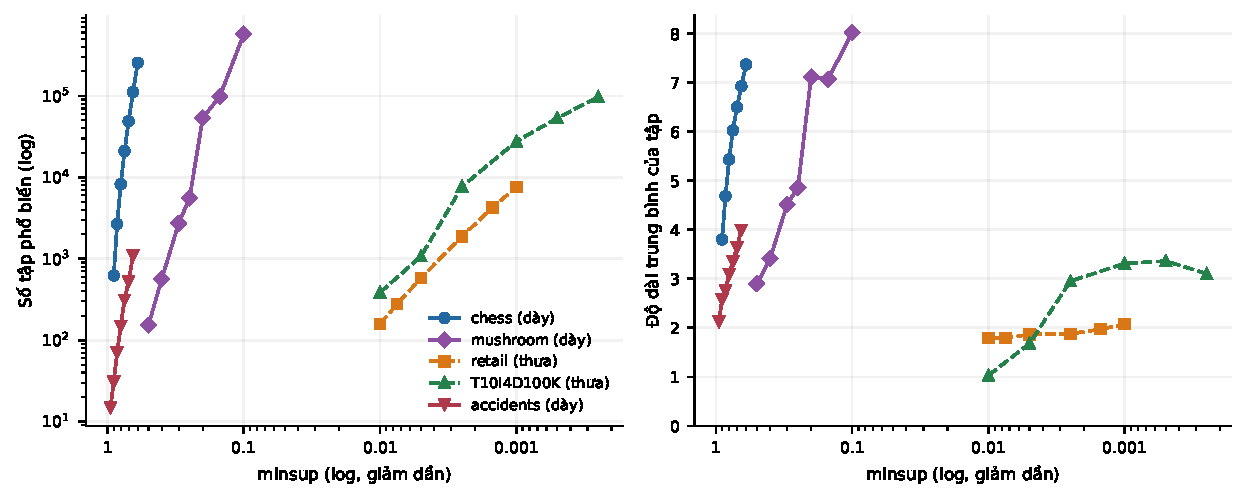
\includegraphics[width=\textwidth]{figures/output-size.pdf}
\caption{Number of frequent itemsets (left, log scale) and mean frequent-itemset length
(right) as minsup decreases on the five databases. Solid lines are dense data and dashed
lines are sparse data.}
\label{fig:output-size}
\end{figure*}

As Fig.~\ref{fig:output-size} shows, the number of frequent itemsets grows much faster on
dense data. The minsup ranges of the five databases differ widely, from a factor of 1.5 on
Chess and Accidents to a factor of 40 on T10I4D100K, and $F$ spans from 15 to
574\,431. To compare growth rates across them, we fit the model
\begin{equation}
  \log F = c - s \log(\mathrm{minsup}),
  \label{eq:output-growth}
\end{equation}
where $F$ is the number of frequent itemsets at a threshold, $c$ is a per-database
constant, and $s$ is the slope on a log-log scale: when minsup falls by a factor $q$, $F$
grows by about $q^s$. Because $s$ depends only on ratios, it can be compared across
databases whose minsup ranges differ. If items occurred independently with probability
$d$, the model would hold with $s \approx \log|I| / \log(1/d)$, which gives 1.5 for
T10I4D100K and 1.3 for Retail, close to the measured 1.6 and 1.7
(Appendix~\ref{app:output-model}). On the dense databases it underestimates $s$, because
their items are correlated, as described below.

The fit is close ($R^2$ between 0.963 and 0.998), but $s$ is an average over each range:
between adjacent thresholds, the slope of Chess falls from 25.5 to 10.4. In
Table~\ref{tab:output-growth}, $s$ ranges from 5.2 to 14.3 on the three dense databases
but is only 1.6 and 1.7 on the two sparse ones. The output of Chess grows 410-fold when
minsup drops merely from 0.9 to 0.6, whereas Retail's grows 48-fold over a tenfold drop.

\begin{table}[t]
\centering
\small
\caption{Number of frequent itemsets $F$ at the highest and lowest threshold, slope $s$
of model~\eqref{eq:output-growth}, and maximum frequent-itemset length $k_{\max}$ at the
lowest threshold}
\label{tab:output-growth}
\setlength{\tabcolsep}{4pt}
\begin{tabular}{lrrrrr}
\hline
Data & minsup & $F$ high & $F$ low & $s$ & $k_{\max}$ \\
\hline
Chess & 0.9--0.6 & 622 & 254\,944 & 14.3 & 14 \\
Accidents & 0.95--0.65 & 15 & 1\,093 & 11.3 & 8 \\
Mushroom & 0.5--0.1 & 153 & 574\,431 & 5.2 & 16 \\
Retail & 0.01--0.001 & 159 & 7\,589 & 1.7 & 5 \\
T10I4D100K & 0.01--0.00025 & 385 & 96\,959 & 1.6 & 11 \\
\hline
\end{tabular}
\end{table}

The difference comes from itemset length. In dense data, each transaction contains a
large share of all items, so many items occur together in most transactions and form long
frequent itemsets. Since a frequent $k$-itemset brings $2^k - 1$ non-empty subsets that
are also frequent, a lower threshold that admits longer itemsets makes the count grow
exponentially in their length. Across the threshold grid, the mean length rises from 3.8
to 7.4 on Chess and from 2.9 to 8.0 on Mushroom. When minsup on Mushroom drops from 0.25
to 0.2, the count grows 9.7-fold, from 5\,545 to 53\,583 itemsets, and the maximum length
jumps from 11 to 15. In sparse data, transactions are short and items rarely occur
together, so lowering the threshold mostly adds single items and pairs. The mean length on
Retail stays between 1.8 and 2.1, and on T10I4D100K 0.00025, 45\,660 of the 96\,959
itemsets (47\%) are 2-itemsets.

The number of frequent itemsets alone does not determine the runtime: the baseline takes
12.59\,s on Retail 0.001 with 7\,589 itemsets but only 3.07\,s on Chess 0.6 with
254\,944, because by~\eqref{eq:cost} the cost depends on the number of intersections
times the tidset length, not on the number of results (Appendix~\ref{app:count-runtime}).

\subsection{Process peak memory}
\label{sec:memory}
The runtime campaign of Section~\ref{sec:minsup} also records the peak RSS of every run,
covering start-up, reading the data, mining, and writing the whole output.
Table~\ref{tab:peak-rss} gives the medians at two thresholds of each database: a medium
minsup, the fourth threshold from the top of its grid in Fig.~\ref{fig:exact-grid}, and
the lowest minsup, where both the output and the search are largest. No run of any program reports less than
252\,MiB, a floor set by the measurement itself. The runner that reads the peak RSS is a
Julia process, and it starts each program by copying itself and then replacing the copy
with the program (\texttt{fork} and \texttt{exec}). On Linux, the peak RSS reported for
the child also counts the copy's resident memory before the replacement, which is the
size of the runner's own Julia runtime. A median at that floor (between 253.3 and
253.6\,MiB) is therefore only an upper bound.

\begin{table}[t]
\centering
\small
\setlength{\tabcolsep}{3pt}
\caption{Median peak RSS (MiB) over five repeats at a medium and at the lowest minsup of
each database. $M_b$ and $M_o$ are the medians of the baseline and the optimized variant,
and ``SPMF'' is SPMF's Eclat. An asterisk marks a median at the measurement floor.}
\label{tab:peak-rss}
\begin{tabular}{lrrrrr}
\hline
Data / minsup & $M_b$ & $M_o$ & $M_b/M_o$ & SPMF & PrePost+ \\
\hline
\multicolumn{6}{l}{\emph{Medium minsup}} \\
Chess / 0.75 & 272.1 & 253.6* & 1.073 & 467.8 & 253.4* \\
Mushroom / 0.25 & 270.3 & 253.5* & 1.066 & 253.4* & 253.4* \\
Retail / 0.0025 & 284.4 & 254.8 & 1.116 & 827.6 & 253.4* \\
T10I4D100K / 0.001 & 282.6 & 261.1 & 1.082 & 380.6 & 285.6 \\
Accidents / 0.8 & 559.3 & 397.3 & 1.408 & 2\,759.0 & 336.6 \\
\hline
\multicolumn{6}{l}{\emph{Lowest minsup}} \\
Chess / 0.6 & 285.1 & 261.5 & 1.090 & 526.5 & 253.4* \\
Mushroom / 0.1 & 366.0 & 299.2 & 1.223 & 514.2 & 253.5* \\
Retail / 0.001 & 289.6 & 280.9 & 1.031 & 844.4 & 253.6* \\
T10I4D100K / 0.00025 & 303.7 & 278.5 & 1.090 & 556.0 & 297.4 \\
Accidents / 0.65 & 608.4 & 398.3 & 1.528 & 4\,248.1 & 340.9 \\
\hline
\end{tabular}
\end{table}

The optimized variant reduces peak memory by $100(1-M_o/M_b)$ percent. At the medium
minsup this ranges from 6.2\% on Mushroom to 29.0\% on Accidents, and where $M_o$ sits at
the floor the true reduction is larger; at the lowest minsup it ranges from 3.0\% on
Retail to 34.5\% on Accidents. SPMF Eclat uses 1.5 to 6.9 times as much memory as the
optimized variant at the medium minsup, apart from Mushroom where both sit at the floor,
and 1.7 to 10.7 times as much at the lowest. PrePost+ uses less on Accidents (336.6 and
340.9 against 397.3 and 398.3\,MiB) and stays at the floor on Chess, Mushroom, and Retail. The optimized variant saves memory with
bitsets and reused buffers (Section~\ref{sec:optimized}). For a database of $N$ transactions, a tidset with $\ell$
tids takes $8\ell$ bytes as a list of 64-bit integers but $8\lceil N/64\rceil$ bytes as a
bit array, counting elements only. The bit array is smaller for long tidsets, and classes
with short tidsets can still switch to lists. Peak RSS, however, also includes the data,
the search structures, the result, and the runtime's own memory, so these numbers show
the difference for the whole process at the chosen thresholds.

\subsection{Scalability}
\label{sec:scalability}
This experiment asks whether runtime grows linearly with the number of transactions $N$
when the database grows and the relative threshold stays fixed. We used Accidents, the
largest database in Table~\ref{tab:datasets}, and Retail, the sparse database with the
most items. Each database was shuffled once with seed 42, and the $p\%$ subset consists of
the first $p\%$ of the shuffled transactions, for $p \in \{10, 25, 50, 75, 100\}$. The
subsets are therefore nested: a larger subset only adds transactions to a smaller one and
never replaces any, so the difference between two points comes entirely from the added
data. The script \texttt{experiments/prepare\_subsets.jl} regenerates the subsets, and
\texttt{data/benchmark/subsets.toml} records the SHA-256 hash of each file. The mean
transaction length barely changes between subsets, staying between 33.79 and 33.81 on
Accidents and between 10.30 and 10.37 on Retail, so sampling preserves the shape of the
data.

The threshold stays at minsup 0.65 for Accidents and 0.001 for Retail, the lowest
threshold of each database in the runtime grid, so the absolute threshold grows with $N$:
from $\sigma_{\min} = 22\,112$ to $221\,119$ on Accidents and from 9 to 89 on Retail. We
timed the four programs through the command line, each run in a fresh process, with five
interleaved repeats. All 200 outputs match an independent SPMF Eclat run exactly, and the
interquartile range stays within 1.9\% of the median for our two variants and within 7.6\%
for the two SPMF programs.

\begin{figure*}[t]
\centering
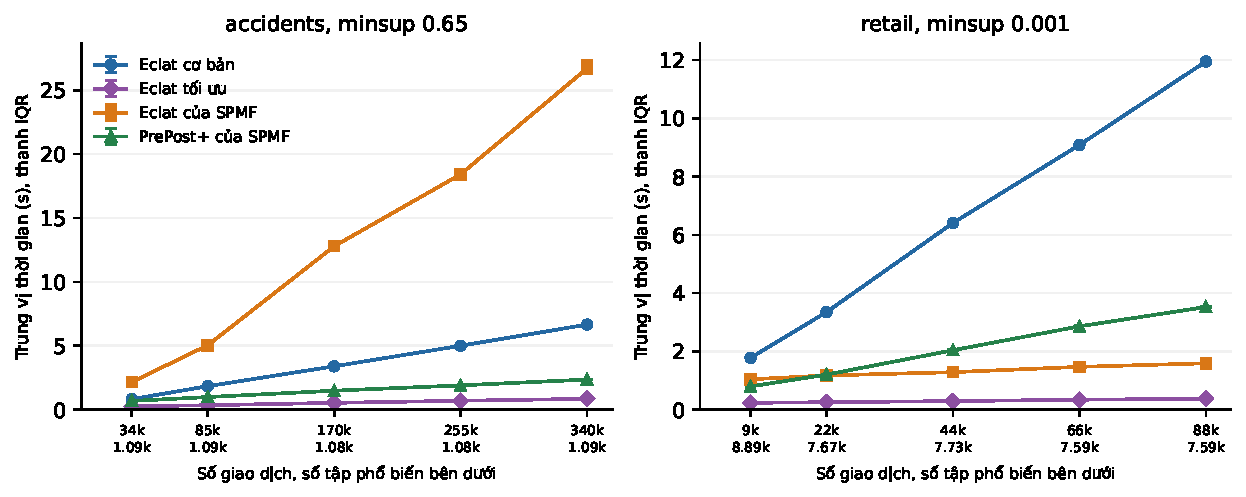
\includegraphics[width=\textwidth]{figures/scalability.pdf}
\caption{Median process time against number of transactions on five nested subsets of
Accidents (minsup 0.65) and Retail (minsup 0.001); error bars are the interquartile range
of five runs. The second row of numbers under the horizontal axis is the number of
frequent itemsets in each subset.}
\label{fig:scalability}
\end{figure*}

All eight lines in Fig.~\ref{fig:scalability} look close to straight. To check this, we
fit each line with the model
\begin{equation}
  T(N) = a + b\,N,
  \label{eq:linear-fit}
\end{equation}
where $T(N)$ is the median time (seconds) on the subset with $N$ transactions, $a$ is a
fixed cost that does not depend on the data, and $b$ is the marginal cost per transaction.
The coefficient of determination $R^2$ is the share of the variance of $T$ that the model
explains; it equals 1 when the five points lie exactly on a line. Every line in
Table~\ref{tab:scalability-fit} has $R^2 \ge 0.992$, so within the measured range the
runtime of all four programs grows linearly with $N$.

\begin{table}[t]
\centering
\small
\caption{Coefficients of model~\eqref{eq:linear-fit}: fixed cost $a$ (s), marginal cost
$b$ (s per 100\,000 transactions), coefficient of determination $R^2$, and the time ratio
between the 100\% and 10\% subsets}
\label{tab:scalability-fit}
\setlength{\tabcolsep}{4pt}
\begin{tabular}{llrrrr}
\hline
Data & Program & $a$ & $b$ & $R^2$ & $T_{100}/T_{10}$ \\
\hline
Accidents & Baseline & 0.19 & 1.90 & 0.9999 & 8.1 \\
 & Optimized & 0.19 & 0.20 & 0.9986 & 3.3 \\
 & SPMF Eclat & $-1.16$ & 8.02 & 0.9951 & 12.3 \\
 & PrePost+ & 0.52 & 0.54 & 0.9987 & 3.5 \\
Retail & Baseline & 0.61 & 12.87 & 0.9996 & 6.7 \\
 & Optimized & 0.22 & 0.18 & 0.9978 & 1.6 \\
 & SPMF Eclat & 1.00 & 0.69 & 0.9923 & 1.5 \\
 & PrePost+ & 0.48 & 3.51 & 0.9983 & 4.4 \\
\hline
\end{tabular}
\end{table}

The complexity bound~\eqref{eq:cost} explains why. With the relative minsup fixed, the
set of frequent itemsets barely changes; Accidents, for instance, has between 1\,079 and
1\,095 frequent itemsets at all five sizes. The search therefore visits the same
equivalence classes, and the number of intersections $C$ stays nearly constant.
Meanwhile, the total length $L$ grows in proportion to $N$, and so does the cost of each
intersection, because a random sample keeps the share of transactions that contain each
itemset nearly the same, so tidsets grow with $N$. With bitsets, an intersection reads
$\lceil N/64 \rceil$ machine words, which is also proportional to $N$. All three terms are
thus linear in $N$, and no step of Eclat depends on the square of the number of
transactions.

The fixed cost $a$ of the optimized variant is 0.19 s on Accidents and 0.22 s on Retail,
close to the Julia start-up and package-loading time reported in Section~\ref{sec:measure}.
Because this fixed part dominates on the small subsets, the optimized variant's time grows
only 3.3-fold on Accidents and 1.6-fold on Retail when $N$ grows tenfold, even though its
line is straight. The coefficient $b$ is the better measure of scalability. The baseline's
marginal cost is 9.7 times the optimized variant's on Accidents and 71 times on Retail. On
Retail, the baseline intersects every pair of frequent items at the root, on tid lists
whose length grows with $N$, which pair counting avoids. As a result, the gap between the two variants widens from a factor of 7.7 on the 10\% subset
to 31.9 on the full database. The optimized variant is also faster than PrePost+ at all
ten points, with $R$ between 0.35 and 0.38 on Accidents and falling from 0.29 to 0.11 on
Retail, because PrePost+ has a marginal cost 2.8 times larger on Accidents and 19 times
larger on Retail.

The number of distinct items and, on Retail 10\%, a very low absolute threshold also
change between subsets, but neither bends the lines: the point farthest from the fitted
line is off by at most 1\% of the full-database time (Appendix~\ref{app:scal-factors}).

SPMF's Eclat is the only program that shows signs of nonlinearity. On Accidents its time
grows 12.3-fold when $N$ grows tenfold, the quadratic term of the fit is positive, and its
$R^2$ of 0.9951 is the lowest of the four Accidents rows. Because the curve bends upward,
the fitted line crosses the vertical axis below zero, so the value of $a$ in that row is
not a fixed cost.

\subsection{Effect of transaction length}
\label{sec:width}
In real benchmarks, transaction length is mixed up with density and output volume. To
isolate it, we generated eight synthetic databases that all have $N = 10\,000$
transactions over $|I| = 100$ items and differ only in the transaction length
$w \in \{5, 10, \dots, 40\}$. Each transaction is a uniformly random subset of exactly $w$
items, drawn independently of the others, so all items are interchangeable and no pair
occurs together more often than chance. A $k$-itemset therefore has expected support
$N \prod_{j=0}^{k-1} (w - j)/(|I| - j)$; a pair, for example, appears in
$N\,w(w-1)/(|I|(|I|-1))$ transactions. The generator uses SplitMix64 with seed
$(42 \ll 32) \,|\, w$ rather than Julia's \texttt{Xoshiro}, because Julia does not promise
the same random stream across versions; this way the SHA-256 hashes in the manifest hold on
every platform.

Two confounding factors still have to be separated. The first is output volume: longer
transactions push more pairs and triples over the threshold, so the number of frequent
itemsets grows in steps, and runtime may follow that count rather than $w$ itself. The
second is co-occurrence, which the model removes by keeping items independent; as a
consequence, the results cannot stand in for the behavior of Chess or Mushroom. We
therefore measure under two protocols. The fixed protocol uses $\mathrm{minsup} = 0.05$ at
every $w$. The matched-output protocol uses, for each $w$, the largest threshold
$\sigma_{\min}$ that still gives at least 5\,000 frequent itemsets, which keeps the output
nearly constant so that $w$ is the only thing that changes.

Under the fixed protocol, the number of frequent itemsets is 53, 100, 100, 100, 5\,050,
5\,050, 5\,050, and 166\,749 as $w$ grows from 5 to 40. Pairs first reach
$\sigma_{\min} = 500$ at $w = 25$ (expected support 606, compared with 384 at $w = 20$),
and triples at $w = 40$ (expected 611). The baseline's runtime follows these steps
(0.42\,s at $w = 20$, 2.27\,s at $w = 25$, and 46.9\,s at $w = 40$ in the \emph{process}
scope, Fig.~\ref{fig:width}), so a plot against $w$ at a single minsup mostly reflects the
output, not the transaction length. As in Section~\ref{sec:minsup}, the \emph{process}
times come from the \texttt{demo.jl} command line at the revision timed there, and all 144
cold attempts of the two protocols match SPMF exactly.

\begin{figure*}[t]
\centering
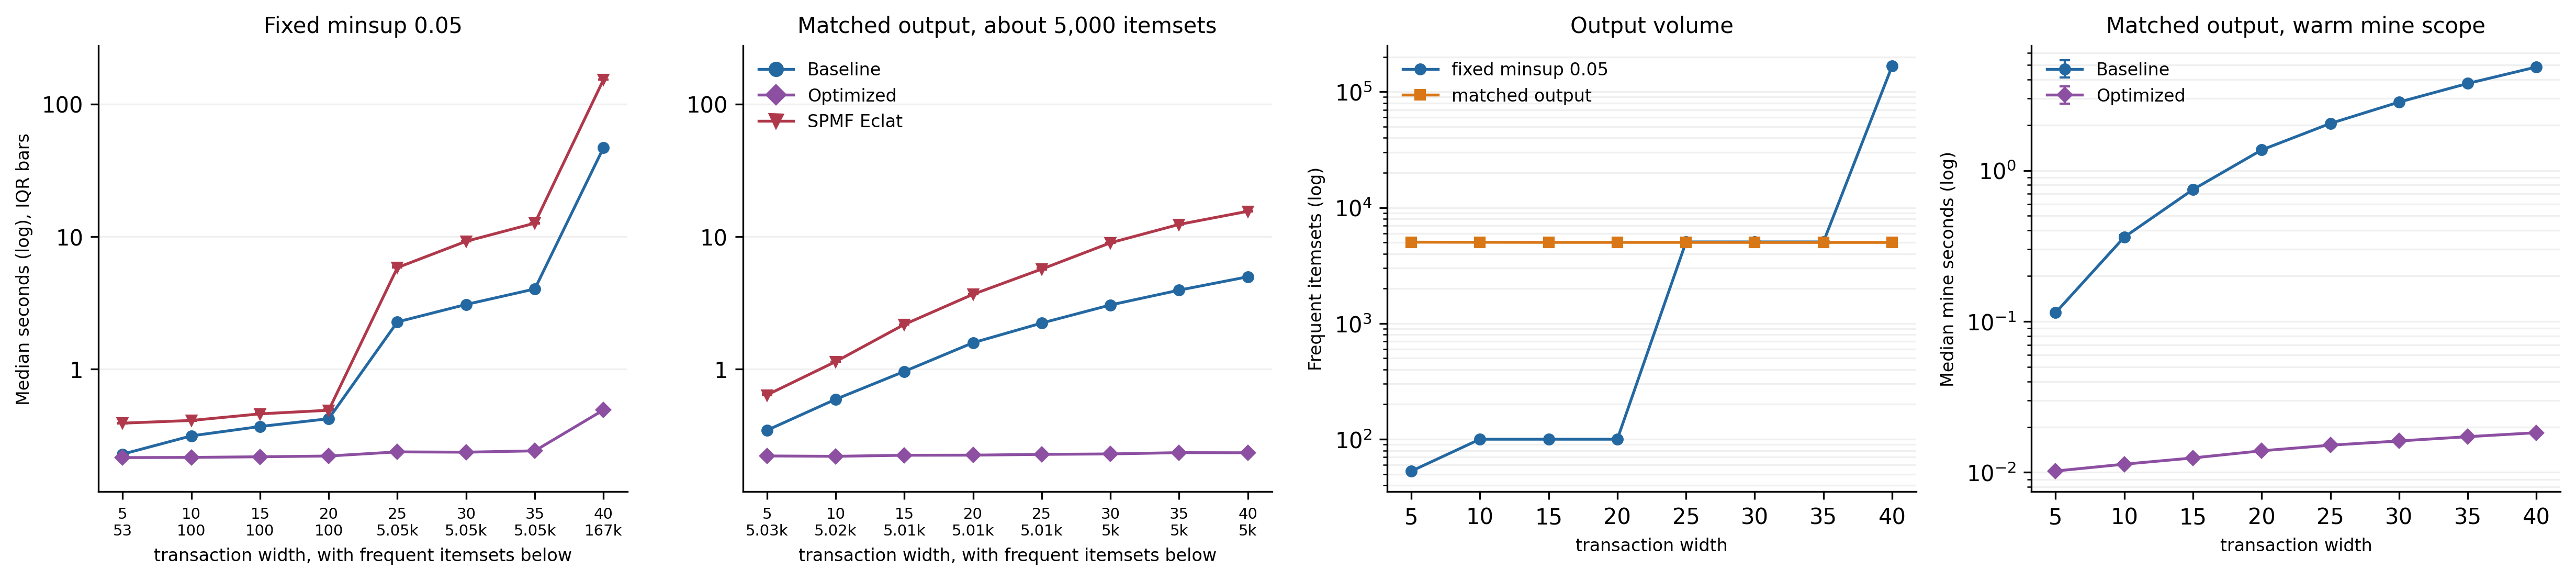
\includegraphics[width=\textwidth]{figures/width-curves.png}
\caption{Runtime and output volume against transaction length $w$ on the synthetic
databases ($N = 10\,000$, $|I| = 100$). From left to right: \emph{process} time at fixed
minsup 0.05; \emph{process} time with output matched to about 5\,000 itemsets; number of
frequent itemsets under both protocols; \emph{mine} time (after warm-up) with matched
output. Medians of three repeats with interquartile-range bars; below each axis label is
the number of frequent itemsets.}
\label{fig:width}
\end{figure*}

Under the matched-output protocol, the number of frequent itemsets stays around 5\,000 and
the number of tidset intersections (joins) is nearly constant, at about 164\,000 with
about 4\,900 successes. Even so, the baseline's mining time grows 42-fold as $w$ goes from
5 to 40 (Table~\ref{tab:width}), because each merge costs time proportional to the
combined length of the two tidsets (Section~\ref{sec:minsup}). Each item appears in a fraction $w/|I|$ of the transactions, so its tidset length
is proportional to $w$, and the tidset of a pair to $w(w-1)$. The total number of merged
elements thus grows 47-fold while $w$ grows only 8-fold, and the baseline's time tracks it
at 9.0 to 10.0\,ns per element. The optimized variant intersects bitsets of
$\lceil N/64 \rceil = 157$ machine words whatever the tidset length, and its mining time
grows only 1.8-fold, from 10.2 to 18.3\,ms; we have not identified where that remaining
growth comes from. In the \emph{process} scope, the optimized variant stays at 0.22 to
0.23\,s, essentially Julia start-up and reading, while the baseline grows 14.4-fold (0.35
to 4.98\,s) and SPMF Eclat 24.3-fold (0.64 to 15.53\,s).

\begin{table}[t]
\centering
\caption{Eclat under the matched-output protocol. $\sigma_{\min}$ is the threshold in
transactions, ``Elements'' is the combined length of the two tidsets over all of the
baseline's intersections, and times are \emph{mine} medians of three repeats.}
\label{tab:width}
\begin{tabular}{rrrrrr}
\hline
$w$ & $\sigma_{\min}$ & Sets & Elements (M) & Baseline (s) & Optimized (ms) \\
\hline
5 & 10 & 5\,028 & 11.4 & 0.114 & 10.2 \\
10 & 69 & 5\,016 & 38.9 & 0.361 & 11.3 \\
15 & 179 & 5\,007 & 82.4 & 0.747 & 12.5 \\
20 & 340 & 5\,007 & 142.0 & 1.366 & 13.9 \\
25 & 550 & 5\,007 & 217.2 & 2.046 & 15.1 \\
30 & 815 & 5\,002 & 308.8 & 2.833 & 16.2 \\
35 & 1\,127 & 5\,002 & 416.4 & 3.765 & 17.2 \\
40 & 1\,488 & 5\,001 & 538.8 & 4.841 & 18.3 \\
\hline
\end{tabular}
\end{table}

These conclusions cover a limited setting: a single $N$ and item count, eight values of
$w$, independent items, and three repeats on one machine. The target of 5\,000 itemsets
is also a choice rather than a derived value. Appendix~\ref{app:width-tree} compares the
search trees of the two protocols.

\subsection{Analysis and future directions}
\label{sec:future}
Two common directions for optimizing Eclat are an adaptive tidset
representation that switches between lists and \emph{bitsets}, and early termination of
tidset intersections. The optimized variant already does both: per-class tid lists, the
early stop in the list merge, and block bounds (Section~\ref{sec:optimized}). Before
proposing anything new, we therefore measured where the optimized variant still
spends its time.

The script \texttt{scripts/stage\_profile.jl} times the three stages of the CLI path,
reading, mining, and writing, in a warm process, taking the median of five runs after one
warm-up run. It also samples the same runs with a \emph{profiler}, a tool that
periodically records which function is running, and assigns each sample to the package
function it falls in. In Table~\ref{tab:stage-profile}, ``Layout'' covers reading the
file, counting items, building the root bitsets, and checking the canonical form;
``Intersect'' covers bitset and list intersections, converting bitsets to lists, block
counting, and search bookkeeping; and ``Output'' covers node expansion, sorting, and
formatting.

\begin{table}[t]
\centering
\footnotesize
\setlength{\tabcolsep}{1.5pt}
\caption{Share of \emph{profiler} samples by group, in percent, for the optimized
variant's CLI path. ``Run'' is the time of one read, mine, and write pass (seconds).
Chess 0.9 and Mushroom 0.5 take only 5 to 7\,ms, too short to sample.}
\label{tab:stage-profile}
\begin{tabular}{lrrrrrr}
\hline
Point & Itemsets & Run & Layout & Pairs & Intersect & Output \\
\hline
Chess 0.6 & 254\,944 & 0.099 & 5 & 0 & 12 & 83 \\
Mushroom 0.1 & 574\,431 & 0.180 & 4 & 0 & 1 & 95 \\
Mushroom 0.05 & 3\,755\,511 & 1.237 & 1 & 0 & 1 & 98 \\
Retail 0.01 & 159 & 0.069 & 98 & 0 & 1 & 0 \\
Retail 0.001 & 7\,589 & 0.144 & 57 & 39 & 4 & 1 \\
T10I4D100K 0.01 & 385 & 0.105 & 66 & 34 & 0 & 0 \\
T10I4D100K 0.00025 & 96\,959 & 0.710 & 10 & 7 & 79 & 5 \\
Accidents 0.95 & 15 & 0.567 & 98 & 0 & 0 & 2 \\
Accidents 0.65 & 1\,093 & 0.619 & 99 & 0 & 0 & 0 \\
\hline
\end{tabular}
\end{table}

Tidset intersection, the core operation of Eclat, takes most of the time at only one
point, T10I4D100K 0.00025. At the three dense points (Chess 0.6 and Mushroom
0.1 and 0.05), output takes 83\% to 98\% of the samples. At the other five points,
building the vertical layout and counting pairs dominate, and on Accidents the search
takes under 1\% of the run. This agrees with the earlier subsections. On Accidents, the
optimized variant's time grows linearly with $N$ while the output stays near 1\,100
itemsets (Section~\ref{sec:scalability}), and its peak RSS exceeds that of the other
databases by roughly the size of the input database itself (105\,MiB by
\texttt{Base.summarysize}). At the dense points, the long itemsets of
Section~\ref{sec:output-size} make the output, not the search, the largest cost. Every
run behind these numbers matches SPMF Eclat exactly.

The strengths and weaknesses relative to SPMF listed below rest on measured behavior
only. On the strong side, the optimized variant's cost per transaction on Accidents is 41 times lower
than SPMF Eclat's and 2.8 times lower than PrePost+'s, and its start-up constant of 0.19
to 0.22\,s is below the 0.48 to 0.52\,s of PrePost+. As transactions grow from 5 to 40
items, its mining time grows only 1.8-fold, because a bitset intersection costs 157 words
at every length (Section~\ref{sec:width}), while SPMF Eclat's \emph{process} time grows
24.3-fold. At the lowest minsup it also needs 1.7 to 10.7 times less memory than SPMF
Eclat (Table~\ref{tab:peak-rss}). On the weak side, Mushroom 0.05 is the only point where the
optimized variant is slower than PrePost+ (1.445 against 1.378\,s). There, output takes
98\% of the run and sorting alone 43\% of the samples, whereas SPMF writes in mining order
and does not sort. On Accidents, PrePost+ also needs 14\% less memory than the optimized
variant (340.9 against 398.3\,MiB).

\paragraph{Proposal 1: a flat integer store and an array-built vertical layout.}
\emph{Bottleneck.} Layout takes 98\% to 99\% of the samples on Accidents and Retail 0.01,
and it drives both the per-transaction slope and the peak RSS discussed above.
\texttt{count\_items} hashes every item occurrence into a \texttt{Dict},
\texttt{bitset\_tidsets} looks up every occurrence in a second \texttt{Dict}, and the
reader allocates a \texttt{Vector} with 8 bytes per item for each transaction.
\emph{Change.} The CLI path would read the database into a single flat \texttt{Int32}
vector plus an offset vector, count items and map them to ranks with an array indexed by
item code, and set the bits from that array. Item codes above a cutoff would still go
through a \texttt{Dict}, and the search itself would not change. \emph{Expected benefit.}
A small prototype that replaced the two \texttt{Dict} passes with array lookups on the
same database cut these two steps on Accidents 0.65 from 0.310 to 0.092\,s (3.4 times
faster, medians of three runs). That saves 35\% of the run on Accidents 0.65, 22\% on
Retail 0.001, and 3\% on T10I4D100K 0.00025. The testable prediction is that the
per-transaction slope on Accidents drops by about a third, while points dominated by
intersection stay the same. Memory should fall as well: the Accidents database takes
105\,MiB as \texttt{Vector\{Vector\{Int\}\}}, 46\,MiB as flat \texttt{Int32}, and
23\,MiB as \texttt{UInt16} (its largest code is 468), a saving of 59 to 82\,MiB out of a
398.3\,MiB peak RSS. The cost is a second reader and layout builder that must stay
equivalent to the general ones; Appendix~\ref{app:proposals} gives the tradeoff and the
tests that would decide whether to keep the change.

\paragraph{Proposal 2: output in search order.}
\emph{Bottleneck.} On Chess 0.6, Mushroom 0.1, and Mushroom 0.05, output takes 83\% to
98\% of the samples, and the lexicographic sort alone takes 35\% to 43\%. Timed directly
in a warm process on the benchmark machine at the same revision (median of seven calls),
computing the sorted order takes 0.025, 0.059, and 0.475\,s at these three points.
Printing in storage order instead of sorted order saves another 0.005, 0.021, and
0.222\,s, because the sorted order reads the result arrays out of sequence.
\emph{Change.} Add an \texttt{order=:search} option to \texttt{write\_itemsets} and an
\texttt{--order search} flag to \texttt{demo.jl} that write itemsets in storage order and
skip the sort. Lexicographic order would remain the default, and neither the search nor
\texttt{SupportMap} would change. \emph{Expected benefit.} Subtracting those warm times
from the \emph{process} medians of Table~\ref{tab:runtime-low} and the stress point, CLI
time on Mushroom 0.05 would drop from 1.445\,s to about 0.97\,s by skipping the sort, or
to 0.75\,s if the result is also read in sequence. The ratio $R$ against PrePost+ would
then fall from 1.05 to between 0.70 and 0.54. We predict an 8\% to 10\% shorter run on
Chess 0.6, 14\% to 20\% on Mushroom 0.1, and no change at the sparse points. The cost is
that files in search order could no longer be compared byte for byte across variants, so
the package keeps the fixed order by default (Appendix~\ref{app:proposals}).

Other directions look less promising on this evidence. More work on adaptive
representations or early termination would pay off only where intersection dominates the
run, and Table~\ref{tab:stage-profile} shows that happening at a single point,
T10I4D100K 0.00025, where the two kinds of intersection take 50\% of the samples and
converting bitsets to lists another 16\%. Diffsets lost to or tied with bitsets at every
point we tested (Section~\ref{sec:measure}). Parallel search over equivalence classes
might help, but we have not measured how evenly the work divides among the root classes,
so we leave it open. Finally, both proposals rest on a profile taken in a warm process
and only on the optimized variant's CLI path, so their benefits remain predictions until
the changes are built and measured.

\section{Ứng dụng thực tế}
\label{sec:applications}
\subsection{Market Basket Analysis — Thien}
\label{sec:basket}
Phân tích giỏ hàng (market basket analysis) tìm các nhóm sản phẩm thường được mua
cùng nhau để nhà bán lẻ sắp xếp, đóng gói hoặc khuyến mãi. Nhóm dùng bộ dữ liệu
Online Retail II~\cite{chen2012}, giấy phép CC BY 4.0, gồm mọi dòng hóa đơn của
một cửa hàng quà tặng trực tuyến tại Anh từ 01/12/2009 đến 09/12/2011. Tệp CSV
được tải từ hai bản sao trên Hugging Face, cố định theo revision; hai bản giống
nhau từng byte và có đúng 1\,067\,371 dòng như UCI công bố. Mã băm SHA-256 của
tệp được kiểm tra trước khi xử lý.

Mỗi giao dịch (transaction) là một hóa đơn (invoice), và mỗi item là một mã sản
phẩm (stock code) viết hoa, vì \texttt{85123a} và \texttt{85123A} chỉ cùng một
sản phẩm. Mã số nguyên của item được gán theo thứ tự mã sản phẩm bằng hàm
\texttt{encode\_transactions}, nên ánh xạ không phụ thuộc thứ tự dòng và đảo ngược
được: tệp \texttt{items.tsv} lưu mã số, mã sản phẩm, mô tả thường gặp nhất và số
giỏ hàng chứa sản phẩm. Bảng~\ref{tab:basket-cleaning} cho thấy tác động của từng
bước làm sạch.

\begin{table}[t]
\centering
\caption{Số dòng và số hóa đơn sau từng bước làm sạch Online Retail II}
\label{tab:basket-cleaning}
\begin{tabular}{lrrr}
\hline
Bước & Bỏ & Còn (dòng) & Hóa đơn \\
\hline
Dữ liệu gốc & & 1\,067\,371 & 53\,628 \\
Dòng trùng lặp & 34\,335 & 1\,033\,036 & 53\,628 \\
Hóa đơn hủy (C) & 19\,104 & 1\,013\,932 & 45\,336 \\
Điều chỉnh nợ xấu (A) & 6 & 1\,013\,926 & 45\,330 \\
Số lượng $\le 0$ & 3\,393 & 1\,010\,533 & 41\,937 \\
Đơn giá $\le 0$ & 2\,621 & 1\,007\,912 & 40\,076 \\
Mã không phải sản phẩm & 4\,555 & 1\,003\,357 & 39\,516 \\
\hline
\end{tabular}
\end{table}

UCI công bố dữ liệu thành hai sheet theo năm, và cả hai đều chứa các ngày 1--9
tháng 12 năm 2010, chiếm 22\,844 trong số 34\,335 dòng trùng. Dòng trùng không làm
thay đổi giỏ hàng vì item lặp lại trong một giao dịch được gộp. Hóa đơn hủy là
hóa đơn riêng mang tiền tố C dùng để đảo một giao dịch bán trước đó, nên bỏ nó
giữ nguyên giỏ hàng khách đã mua. Các dòng có số lượng hoặc đơn giá không dương là
ghi chú kho như ``check'' hay ``damaged'', không phải giao dịch bán; hai bước này
bỏ 5\,254 hóa đơn chỉ gồm ghi chú và 380 mã chưa từng được bán. Bước cuối bỏ các
mã dịch vụ như phí vận chuyển, giảm giá, phí ngân hàng và phiếu quà tặng; riêng
phí vận chuyển xuất hiện trong 8,8\% số hóa đơn nên sẽ tạo luật giả với mọi sản
phẩm phổ biến. Dòng không có mã khách hàng vẫn được giữ vì một hóa đơn là một giỏ
hàng bất kể ai trả tiền.

Kết quả gồm 39\,516 giỏ hàng trên 4\,725 sản phẩm. Độ dài giỏ hàng có trung vị
15, phân vị 90 là 51, trung bình 25,1 và lớn nhất 1\,106 ở các đơn bán sỉ; 92\%
số giỏ hàng đến từ Anh. Với Eclat của nhóm, minsup 0,01 (396 hóa đơn) cho
1\,355 tập phổ biến, trong đó 648 tập có từ hai sản phẩm trở lên.

\subsubsection{Luật kết hợp}
Một luật kết hợp (association rule) $X \Rightarrow Y$ gồm vế trái (antecedent)
$X$ và vế phải (consequent) $Y$ là hai tập sản phẩm khác rỗng, rời nhau. Gọi
$N$ là số giỏ hàng và $\sigma(Z)$ là số giỏ hàng chứa mọi sản phẩm của tập $Z$.
Ba độ đo của luật là
\begin{align}
\mathrm{supp}(X \Rightarrow Y) &= \frac{\sigma(X \cup Y)}{N}, \label{eq:rule-supp}\\
\mathrm{conf}(X \Rightarrow Y) &= \frac{\sigma(X \cup Y)}{\sigma(X)}, \label{eq:rule-conf}\\
\mathrm{lift}(X \Rightarrow Y) &= \frac{\mathrm{conf}(X \Rightarrow Y)}{\sigma(Y)/N}
  = \frac{N\,\sigma(X \cup Y)}{\sigma(X)\,\sigma(Y)}. \label{eq:rule-lift}
\end{align}
Độ hỗ trợ (support)~\eqref{eq:rule-supp} là tỉ lệ giỏ hàng chứa cả hai vế; độ
tin cậy (confidence)~\eqref{eq:rule-conf} là tỉ lệ giỏ hàng có $X$ cũng có $Y$;
độ nâng (lift)~\eqref{eq:rule-lift} cho biết $Y$ đi cùng $X$ nhiều gấp bao nhiêu
lần so với khi hai vế độc lập, nên lift lớn hơn 1 nghĩa là hai vế hay được mua
cùng nhau. Lift đối xứng theo $X$ và $Y$, còn độ tin cậy thì không.

Nhóm khai thác 39\,516 giỏ hàng bằng Eclat của nhóm với minsup 0,01, tức mỗi
mẫu dựa trên ít nhất 396 hóa đơn, và nhận 1\,355 tập phổ biến. Mỗi tập phổ biến
$Z$ có $m \ge 2$ sản phẩm được tách thành mọi cặp $X$, $Y = Z \setminus X$, tức
$2^m - 2$ luật; ngưỡng minsup đã áp lên $X \cup Y$ khi khai thác, và mọi tập con
của $Z$ đều có trong kết quả nên $\sigma(X)$, $\sigma(Y)$ luôn tra được. Các độ
đo được tính bằng phân số chính xác. Ngưỡng minconf được đổi một lần từ dạng
thập phân thành phân số $p/q$, và luật được giữ khi
$\sigma(X \cup Y)\, q \ge p\, \sigma(X)$, tính bằng số nguyên cỡ lớn, nên sai số
làm tròn không quyết định luật nào. Cách so sánh với số thực 0,1 trong máy, lớn
hơn $1/10$ một chút, sẽ loại nhầm luật có độ tin cậy đúng bằng $1/10$. Với
minconf 0,5, 455 trong 1\,804 luật được giữ lại, và mọi luật có lift trên 1,4.

Để kiểm tra, nhóm chạy Eclat của SPMF trên cùng tệp giỏ hàng: hai kết quả khớp
100\% trên 1\,355 tập phổ biến. Một chương trình riêng sinh luật từ kết quả của
SPMF cũng cho đúng 455 luật, và độ hỗ trợ, độ tin cậy, lift của 10 luật đứng đầu
khớp với phép đếm trực tiếp trên giỏ hàng.

Luật được xếp theo lift giảm dần, rồi độ tin cậy, rồi số giỏ hàng, cuối cùng
theo mã sản phẩm, để thứ tự luôn xác định. Hai luật $X \Rightarrow Y$ và
$Y \Rightarrow X$ luôn bằng lift nên hướng có độ tin cậy cao hơn đứng trước.
Bảng~\ref{tab:top-rules} liệt kê 10 luật đứng đầu; không luật nào ngoài bảng có
lift bằng luật thứ 10.

\begin{table}[t]
\centering
\caption{10 luật có lift cao nhất (minsup 0,01, minconf 0,5). B, K, L là bộ
Poppy's Playhouse Bedroom, Kitchen, Livingroom; $\sigma$ là số giỏ hàng chứa cả
hai vế}
\label{tab:top-rules}
\begin{tabular}{rlrrrr}
\hline
Hạng & Luật & $\sigma$ & supp & conf & lift \\
\hline
1 & B + K $\Rightarrow$ L & 409 & 0,0104 & 0,734 & 51,45 \\
2 & L $\Rightarrow$ B + K & 409 & 0,0104 & 0,725 & 51,45 \\
3 & L + K $\Rightarrow$ B & 409 & 0,0104 & 0,863 & 48,50 \\
4 & B $\Rightarrow$ L + K & 409 & 0,0104 & 0,582 & 48,50 \\
5 & B + L $\Rightarrow$ K & 409 & 0,0104 & 0,887 & 47,25 \\
6 & K $\Rightarrow$ B + L & 409 & 0,0104 & 0,551 & 47,25 \\
7 & L $\Rightarrow$ B & 461 & 0,0117 & 0,817 & 45,95 \\
8 & B $\Rightarrow$ L & 461 & 0,0117 & 0,656 & 45,95 \\
9 & L $\Rightarrow$ K & 474 & 0,0120 & 0,840 & 44,76 \\
10 & K $\Rightarrow$ L & 474 & 0,0120 & 0,639 & 44,76 \\
\hline
\end{tabular}
\end{table}

Cả 10 luật đều thuộc một dòng sản phẩm: sáu cách tách của tập ba phòng đồ chơi
Poppy's Playhouse và hai cặp luật đối xứng. Một tập phổ biến sinh nhiều luật gần
giống nhau, nên Bảng~\ref{tab:top-groups} chỉ giữ luật tốt nhất của mỗi nhóm sản
phẩm $X \cup Y$ khác nhau.

\begin{table*}[t]
\centering
\caption{Luật tốt nhất của 10 nhóm sản phẩm có lift cao nhất, cùng lift khi đếm
lại trong từng năm và khi bỏ 1\% giỏ hàng lớn nhất}
\label{tab:top-groups}
\begin{tabular}{rlrrrrrr}
\hline
 & Luật & $\sigma$ & conf & lift & lift năm 1 & lift năm 2 & lift bỏ giỏ lớn \\
\hline
1 & Poppy's Playhouse Bedroom + Kitchen $\Rightarrow$ Livingroom & 409 & 0,734 & 51,4 & 63,4 & 43,1 & 57,4 \\
2 & Poppy's Playhouse Livingroom $\Rightarrow$ Bedroom & 461 & 0,817 & 45,9 & 60,1 & 37,1 & 52,3 \\
3 & Poppy's Playhouse Livingroom $\Rightarrow$ Kitchen & 474 & 0,840 & 44,8 & 58,0 & 36,2 & 50,3 \\
4 & Poppy's Playhouse Bedroom $\Rightarrow$ Kitchen & 557 & 0,792 & 42,2 & 56,2 & 33,6 & 48,4 \\
5 & Wooden Tree $\Rightarrow$ Wooden Star Christmas Scandinavian & 437 & 0,790 & 40,7 & 56,0 & 32,1 & 46,6 \\
6 & Small Marshmallows Pink Bowl $\Rightarrow$ Small Dolly Mix Orange Bowl & 457 & 0,744 & 40,1 & 62,0 & 29,3 & 48,4 \\
7 & Set/10 Blue Spotty $\Rightarrow$ Pink Polkadot Party Candles & 488 & 0,776 & 38,0 & 33,2 & 44,3 & 40,3 \\
8 & Key Fob Garage Design $\Rightarrow$ Key Fob Back Door & 402 & 0,646 & 37,1 & 33,8 & 41,1 & 42,4 \\
9 & Feltcraft Princess Lola $\Rightarrow$ Princess Charlotte Doll & 401 & 0,620 & 35,8 & 52,2 & 27,2 & 39,1 \\
10 & Pink Polkadot Cup $\Rightarrow$ Blue Polkadot Cup & 521 & 0,694 & 35,6 & 31,3 & 41,2 & 39,3 \\
\hline
\end{tabular}
\end{table*}

\subsubsection{Ý nghĩa kinh doanh}
Các nhóm trong Bảng~\ref{tab:top-groups} gợi ý hai giả thuyết có thể hành động.
Thứ nhất, khách mua trọn bộ sưu tập: ba phòng Poppy's Playhouse, hai mẫu búp bê
Feltcraft và hai món trang trí Giáng sinh kiểu Scandinavia. Trong 82\% giỏ hàng
có phòng Livingroom cũng có phòng Bedroom, nên cửa hàng có thể bán theo bộ, đặt
các món cạnh nhau trên trang sản phẩm, hoặc gợi ý món còn thiếu khi giỏ hàng mới
có một phòng. Thứ hai, khách mua nhiều biến thể màu của cùng một sản phẩm: nến
tiệc xanh và hồng, cốc chấm bi hồng và xanh, móc khóa hai kiểu. Cửa hàng có thể
bán gói nhiều màu và nhập hàng các biến thể cùng lúc. Bằng chứng cho cả hai là
lift trên 35, độ tin cậy từ 0,62 đến 0,84 và hơn 400 hóa đơn cho mỗi nhóm.

Luật kết hợp chỉ cho biết hai sản phẩm xuất hiện cùng hóa đơn, không cho biết
mua $X$ là nguyên nhân mua $Y$. Nhiều khách hàng là nhà bán sỉ, nên một nguyên
nhân chung, như việc nhập cả dòng sản phẩm cho cửa hàng của họ hay mùa Giáng
sinh, có thể tạo ra cả hai vế. Vì vậy các gợi ý trên là giả thuyết cần kiểm
chứng, chẳng hạn bằng thử nghiệm A/B cho gói sản phẩm, trước khi thay đổi cách
bán hàng.

\subsubsection{Độ vững của kết quả}
Lift và độ tin cậy là tính chất của dữ liệu, nên thay đổi ngưỡng chỉ quyết định
luật nào được giữ và luật đó được xếp hạng cùng những luật nào. Khi tăng minconf
lên 0,6, hai luật có độ tin cậy 0,58 và 0,55 bị loại khỏi Bảng~\ref{tab:top-rules}
nhưng cả 10 nhóm vẫn còn. Khi giảm minsup xuống 0,0075, mọi luật vẫn còn nhưng
các luật hiếm hơn có lift cao hơn đẩy 10 nhóm xuống hạng 32 đến 108. Khi tăng
minsup lên 0,015 (593 hóa đơn), cả 10 nhóm biến mất vì chúng chỉ có 401 đến 557
hóa đơn: các mẫu có lift cao nhất nằm sát ngưỡng hỗ trợ.

Để phân biệt mẫu vững với mẫu ngẫu nhiên, nhóm đếm lại mỗi luật trong năm thứ
nhất (trước 01/12/2010, 19\,743 giỏ hàng), năm thứ hai (19\,773 giỏ hàng) và
khi bỏ 393 giỏ hàng có hơn 197 sản phẩm, tức 1\% giỏ hàng lớn nhất. Nhóm đếm
trực tiếp thay vì khai thác lại, vì khai thác một nửa dữ liệu với cùng minsup
tương đối sẽ loại những mẫu chỉ hơi dưới ngưỡng mới và trông như mẫu đã biến
mất. Bảng~\ref{tab:top-groups} cho thấy mọi nhóm giữ lift trên 27 và độ tin cậy
từ 0,62 đến 0,90 trong mọi tập con, với ít nhất 108 hóa đơn mỗi năm, nên chúng
không phải sản phẩm của một mùa hay của vài đơn bán sỉ lớn.

Ngược lại, ở minsup 0,005 (198 hóa đơn), chín trong mười nhóm đứng đầu là bộ
nhãn cắm cây gia vị (Herb Marker) với lift khoảng 150. Năm thứ nhất chỉ có 7 đến
11 hóa đơn của mỗi nhóm, khiến lift của năm đó lên tới 1\,480--1\,795 và không
còn ý nghĩa, còn năm thứ hai có 193 đến 221 hóa đơn. Những luật này dựa trên
khoảng một nửa số hóa đơn của các nhóm chính và chủ yếu trên một mùa bán hàng,
nên nhóm xem chúng là hướng cần theo dõi, không phải kết luận.

\subsubsection{Giới hạn}
Dữ liệu đến từ một cửa hàng quà tặng trực tuyến trong hai năm, 92\% hóa đơn ở
Anh và nhiều khách là nhà bán sỉ, nên các luật không đại diện cho bán lẻ nói
chung. Giỏ hàng chỉ ghi sản phẩm có mặt, bỏ qua số lượng và giá, nên một hóa
đơn mua một chiếc và một hóa đơn mua trăm chiếc có trọng số như nhau. Lift ưu
tiên các sản phẩm ít gặp, vì vậy bảng xếp hạng theo lift cần đọc cùng số hóa
đơn hỗ trợ. Cuối cùng, mô tả sản phẩm là nhãn do cửa hàng nhập, có thể khác nhau
giữa các mã gần giống nhau.
\subsection{Khai thác mẫu hình ảnh}
\label{sec:visual-patterns}
\subsubsection{Từ ảnh đến giao dịch}
Bộ dữ liệu Semeion từ UCI gồm 1.593 ảnh chữ số viết tay nhị phân kích thước
$16\times16$ pixel, có nhãn từ 0 đến 9~\cite{semeionUCI}. Câu hỏi khảo sát là
những tổ hợp nét cục bộ nào lặp lại giữa các ảnh. Biểu diễn \emph{bag of
visual words} (túi từ thị giác) đưa mỗi ảnh về một tập mục để Eclat đếm số ảnh
chứa từng tổ hợp nét. Nhóm chia ảnh thành 16 mảnh $4\times4$ không chồng lấp.
Mỗi mảnh ảnh (patch) có ít nhất hai pixel nét được trải theo hàng thành
vector nhị phân 16 chiều. Nhóm dùng k-means với seed (hạt giống ngẫu nhiên)
42 và tối đa 25 vòng lặp để học codebook (từ điển mã) mặc định gồm 24 tâm cụm.
Mỗi tâm là một từ thị giác. Một patch được gán vào tâm gần nhất nếu khoảng
cách Euclid bình phương không vượt quá 1,0. Giao dịch ảnh lưu mỗi từ được
gán đúng một lần, nên vị trí và số lần lặp của patch không tham gia vào support.
Lưới $4\times4$ giữ được các đoạn nét cục bộ trong khi giới hạn mỗi ảnh ở
16 patch trước lọc. Ngưỡng khoảng cách loại các patch ở xa mọi tâm cụm để
hạn chế gán các hình nét khác biệt vào cùng một từ.

Trong số 18.386 patch qua bước lọc pixel nét, các patch đạt ngưỡng khoảng cách
tạo 5.767 lượt hiện diện từ, trung bình 3,62 từ mỗi ảnh. Giao dịch chứa từ 0
đến 8 từ, trung vị là 4. Nhóm giữ 11 giao dịch rỗng trong mẫu số khi đổi minsup
sang ngưỡng nguyên theo Mục~\ref{sec:protocol}. Tệp \texttt{visual\_words.svg}
lưu patch quan sát đại diện cho từng tâm. Tệp \texttt{manifest.toml} lưu seed,
tham số và mã băm đầu vào để tái lập bộ mã hóa. Nhóm học từ điển trên toàn bộ
Semeion để phân tích mô tả.

\subsubsection{Mẫu phổ biến và ảnh hỗ trợ}
Nhóm khai thác các giao dịch bằng Eclat cơ bản của nhóm. Với 24 từ và minsup
20\%, 10\% và 5\%, toàn bộ 6, 18 và 46 tập mục tương ứng khớp support với
SPMF. Đầu vào SPMF có 1.582 giao dịch sau khi bỏ 11 dòng rỗng. Nhóm điều chỉnh
ngưỡng tương đối của SPMF để giữ nguyên số ảnh tối thiểu lần lượt là 319, 160
và 80. Giao dịch rỗng không đóng góp support cho tập mục khác rỗng.

Bảng~\ref{tab:image-evidence} trình bày ba mẫu ở minsup 5\%. Từ 13 có patch
đại diện là nét ngang ngắn. Mẫu $\{8,13\}$ mô tả các ảnh đồng thời chứa patch
của hai cụm. Tệp \texttt{supporting\_images.tsv} liệt kê ID và nhãn của từng
ảnh hỗ trợ. Nhóm đối chiếu ảnh có cùng nhãn để diễn giải sự khác biệt ở mức
patch. Trong Hình~\ref{fig:semeion-contrast}, hai ảnh đều mang nhãn chữ số 2.
Ảnh 44 có cả ba từ. Ảnh 41 có từ 8 và 13 nhưng thiếu từ 4.

\begin{table}[ht]
\centering
\caption{Support và ID ảnh minh họa cho ba mẫu thị giác ở minsup 5\%}
\label{tab:image-evidence}
\begin{tabular}{l r l l}
\hline
Tập từ & Support & Khớp & Không khớp \\
\hline
\{13\} & 863 & 2, 3, 4 & 1, 5, 7 \\
\{8,13\} & 330 & 3, 11, 41 & 2, 4, 6 \\
\{4,8,13\} & 90 & 44, 46, 61 & 41, 42, 43 \\
\hline
\end{tabular}
\end{table}

\begin{figure}[t]
\centering
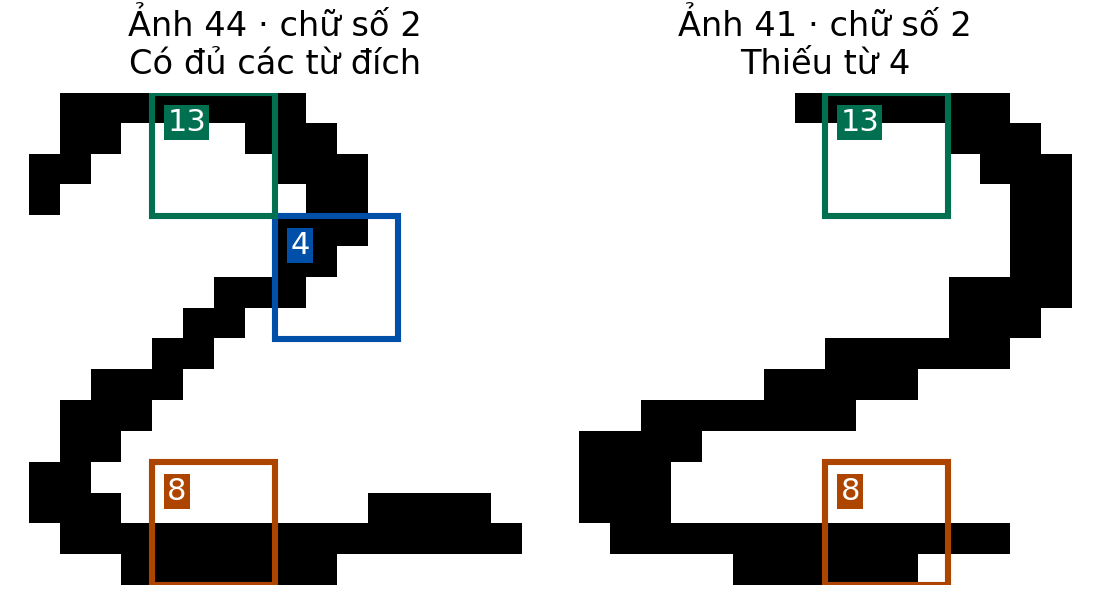
\includegraphics[width=\columnwidth]{figures/semeion-source-contrast.png}
\caption{Hai ảnh nguồn cùng nhãn chữ số 2. Các ô đánh dấu patch được gán
vào từ tương ứng. Ảnh 44 chứa đủ bộ ba $\{4,8,13\}$. Ảnh 41 thiếu từ 4.}
\label{fig:semeion-contrast}
\end{figure}

\subsubsection{Độ nhạy theo từ điển và minsup}
Bảng~\ref{tab:semeion-sensitivity} so sánh số tập mục theo kích thước từ điển
$K$ và minsup, với cùng seed, lưới patch, số vòng lặp tối đa và ngưỡng khoảng
cách. Số ảnh rỗng là số ảnh không có patch được gán từ. Với $K=24$, từ 13 và
cặp $\{8,13\}$ đạt cả năm ngưỡng. Bộ ba $\{4,8,13\}$ có support 90, đạt
ngưỡng 5,5\% (88 ảnh) và nằm dưới ngưỡng 6\% (96 ảnh).

\begin{table}[t]
\centering
\caption{Số tập mục theo kích thước từ điển $K$ và minsup trên Semeion}
\label{tab:semeion-sensitivity}
\begin{tabular}{rrrrrrr}
\hline
$K$ & Ảnh rỗng & 20\% & 10\% & 6\% & 5,5\% & 5\% \\
\hline
16 & 99 & 4 & 12 & 19 & 21 & 25 \\
24 & 11 & 6 & 18 & 35 & 43 & 46 \\
32 & 2 & 5 & 24 & 45 & 52 & 63 \\
\hline
\end{tabular}
\end{table}

Khi $K$ tăng từ 16 lên 32, độ rộng trung bình tăng từ 2,27 lên 4,31 từ mỗi
ảnh. Ở ngưỡng 20\%, từ điển 24 từ cho nhiều mẫu nhất trong ba cấu hình.
Tâm cụm được học lại ở mỗi $K$, nên cần so patch đại diện khi diễn giải từ
giữa các cấu hình. Mức phổ biến của một nét còn phụ thuộc vào cách đặt lưới
và độ phân giải của ảnh nhị phân.

\subsubsection{Ứng dụng và giới hạn}
Mẫu thị giác có thể làm truy vấn theo tổ hợp nét. Chẳng hạn, truy vấn
$\{8,13\}$ trả về 330 ảnh. Khi chuẩn hóa theo số ảnh mỗi nhãn, mẫu này có mặt
ở 69/159 ảnh chữ số 3 (43,4\%) và 9/161 ảnh chữ số 4 (5,6\%). Chênh lệch
mô tả tần suất theo nhãn trong chính bộ dữ liệu dùng để học từ điển. Hai từ
có thể hiện diện ở các vị trí bất kỳ trong ảnh.

Mỗi tập mục cũng có thể tạo một đặc trưng nhị phân. Với danh sách mẫu
$(\{13\},\{8,13\},\{4,8,13\})$, ảnh có giao dịch $\{8,13\}$ nhận vector
$(1,1,0)$. Notebook tạo ma trận gồm 1.593 hàng ảnh và 46 cột tập mục ở minsup
5\%. Tổng mỗi cột bằng support của tập mục tương ứng. Để đánh giá hiệu quả
phân loại của đặc trưng này, cần học từ điển và khai thác mẫu trên tập huấn
luyện, rồi giữ cố định cả hai khi mã hóa tập kiểm tra. Phân tích ở đây mô tả
tần suất trên Semeion.

\href{https://github.com/NgTHung/Itemset/blob/main/notebooks/demo.ipynb}
{Notebook của repository} dùng Julia 1.13.2 và seed 42 để tái lập pipeline
mặc định. Manifest của lượt chạy ghi revision, seed và mã băm của từ điển
cùng đầu ra tại minsup 20\%, 10\% và 5\%. Lưới trong
Bảng~\ref{tab:semeion-sensitivity} dùng cùng bộ mã hóa ở 15 cấu hình.

\bibliographystyle{IEEEtran}
\bibliography{references}
\end{document}
